\chapter{Istniejące rozwiązania}


  W tym rozdziale zostanie przeprowadzona analiza rynku oprogramowania wspierającego fazę analizy. Druga część rozdziału zajmie się identyfikacją najistotniejszych problemów jakie posiadają istniejące rozwiązania. 

  Ilość aplikacji związanych z procesami inżynierii wymagań dostępnych na rynku jest ogromna. Zestawienie INCOSE Requirements Management Tools Survey \cite{Incose} zawiera podzbiór tych narzędzi, jednak opublikowana lista nie jest od dawna aktualizowana, oraz nie wprowadza żadnego rodzaju kategoryzacji. 

  \section{Analiza rynku systemów wsparcia zbierania wymagań}

    Jak wspomniano we wstępnie do rozdziału, na rynku nie brakuje systemów wsparcia procesu zbierania wymagań. Dostępne rozwiązania oferowane są w zasadzie w trzech różnych modelach. Najpopularniejszą ostatnio architekturą jest Software As A Service, czyli aplikacja internetowa zainstalowana na serwerach twórcy oprogramowania lub w infrastrukturze zewnętrznej firmy hostingowej. 
    
    Również klasyczne aplikacje okienkowe, które należy zainstalować na komputerze klienta nadal cieszą się dużą popularnością. Należy jednak zaznaczyć, iż w często są to starsze systemy, nierzadko implementowane jeszcze przed popularyzacją zaawansowanych aplikacji webowych. Niektóre firmy oferują także platformy w architekturze klient-serwer, wymagające istnienia zarówno centralnego serwera - repozytorium w sieci jak i desktopowych aplikacji klienckich. W tej sekcji zostaną przedstawione i porównane wybrane aplikacje z każdej z trzech kategorii. 

    \subsection{Model SaaS (Software as a Service)}

      W ostatnim czasie, wraz z popularyzacją i rozwojem technologii internetowych znacznie wzrosły techniczne możliwości aplikacji dostępnych z poziomu przeglądarki internetowej. Tendencja ta sprzyja powstawaniu licznych aplikacji, adresujących specyficzne problemy, często w obrębie ściśle określonego segmentu rynku. Jednym z przykładów takiego wąskiego segmentu mogą być np. aplikacje do zarządzania projektami online. Wśród popularnych rozwiązań znajdują się takie produkty jak basecamp.com unfuddle.com czy polski nozbe.com. Innym przykładem mogą być aplikacje wspierające proces rekrutacji (humanway.com, recruiterbox.com, jobvite.com). Na uwagę zasługują także aplikacje wspierające rezerwacje hoteli, pensjonatów i niezależnych pokoi i mieszkań jak airbnb.com, booking.com czy b\&b.com. 

      Naturalnie powyższe przykłady dotyczą tylko skrawka możliwych do zagospodarowania segmentów. W rzeczywistości, bardzo ciężko znaleźć wertykalny rynek, który jest niezagospodarowany serwisami, oferującymi różne podejścia do rozwiązania problemów z danej dziedziny. 

      Powodem takiego stanu rzeczy jest szeroko pojęta popularyzacja internetu oraz sukcesywne przenoszenie się do sieci firm tworzących opgrogramowanie. Dystrybucja oprogramowania w formule SaaS ma wiele zalet w stosunku do klasycznych aplikacji "desktopowych". W szczególności pominięty jest w tym przypadku proces rozprowadzania aplikacji do klientów za pomocą sieci stacjonarnych sklepów z oprogramowaniem, jak miało to miejsce w ciągu ostatniej dekady. Zaimplementowane rozwiązanie, jest gotowe do użycia z chwilą udostępnienia w internecie. Udostępnienie aplikacji na serwerach twórcy oprogramowania lub takich dostarczycieli usług jak Amazon Web Services czy Heroku, daje nieograniczone możliwości wprowadzania nowych funkcjonalności, poprawek i skalowania systemu. Z kolei monitorowanie zachowań klientów pozwala niemalże w czasie rzeczywistym odpowiadać na potrzeby użytkowników poprzez modyfikację i wdrażanie nowych funkcjonalności. 

      W związku z licznymi zaletami modelu SaaS, w internecie powstało wiele aplikacji próbujących zaadresować problemy związane z procesem zbierania i dokumentowania wymagań użytkownika. Do najciekawszych rozwiązań można zaliczyć gatherspace.com, accompa.com, requirementone.com, tracecloud.com czy Jama Contour (http://www.jamasoftware.com/contour/)
    
      Na potrzeby tej pracy zostaną przedstawione funkcjonalności systemów Gatherspace oraz Tracecloud.

      \begin{figure*}[t]
        \centering
        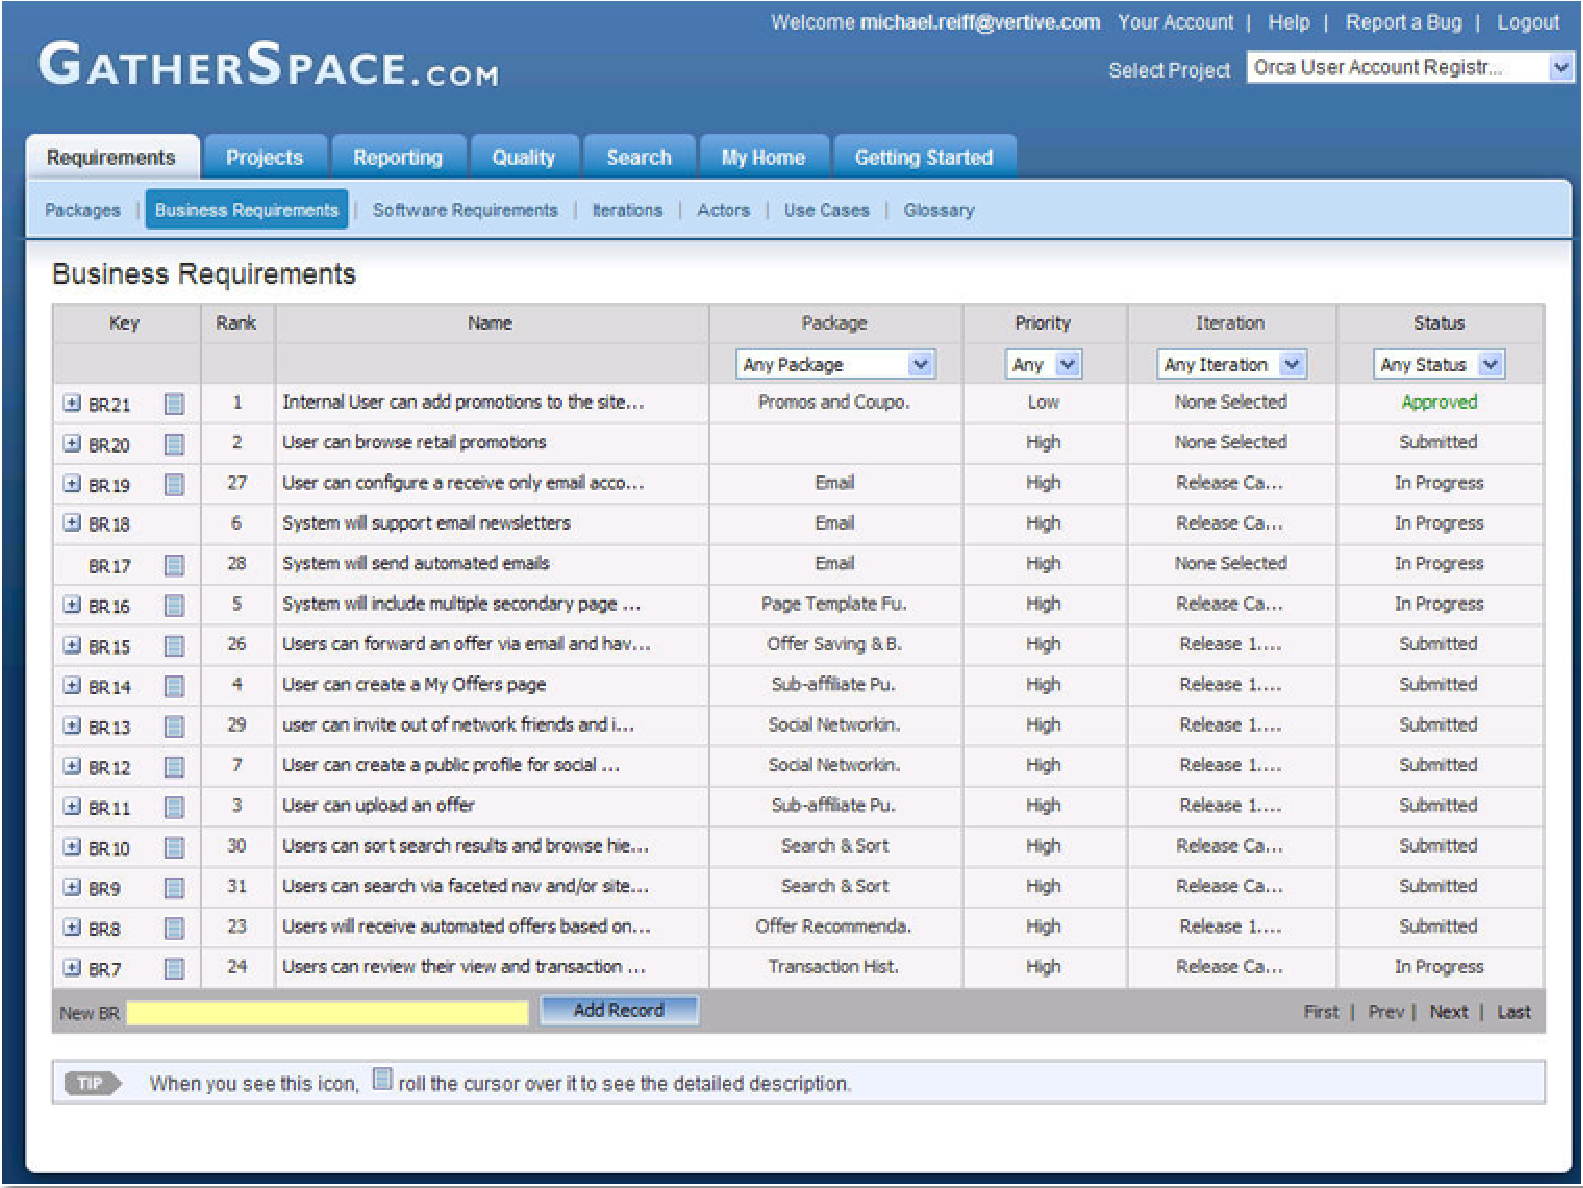
\includegraphics[width=1.0\textwidth]{img/gatherspace_1.pdf}
        \caption{Gatherspace.com - business requirements}
        \label{fig:gatherspace_1}
      \end{figure*}

      \begin{figure*}[t]
        \centering
        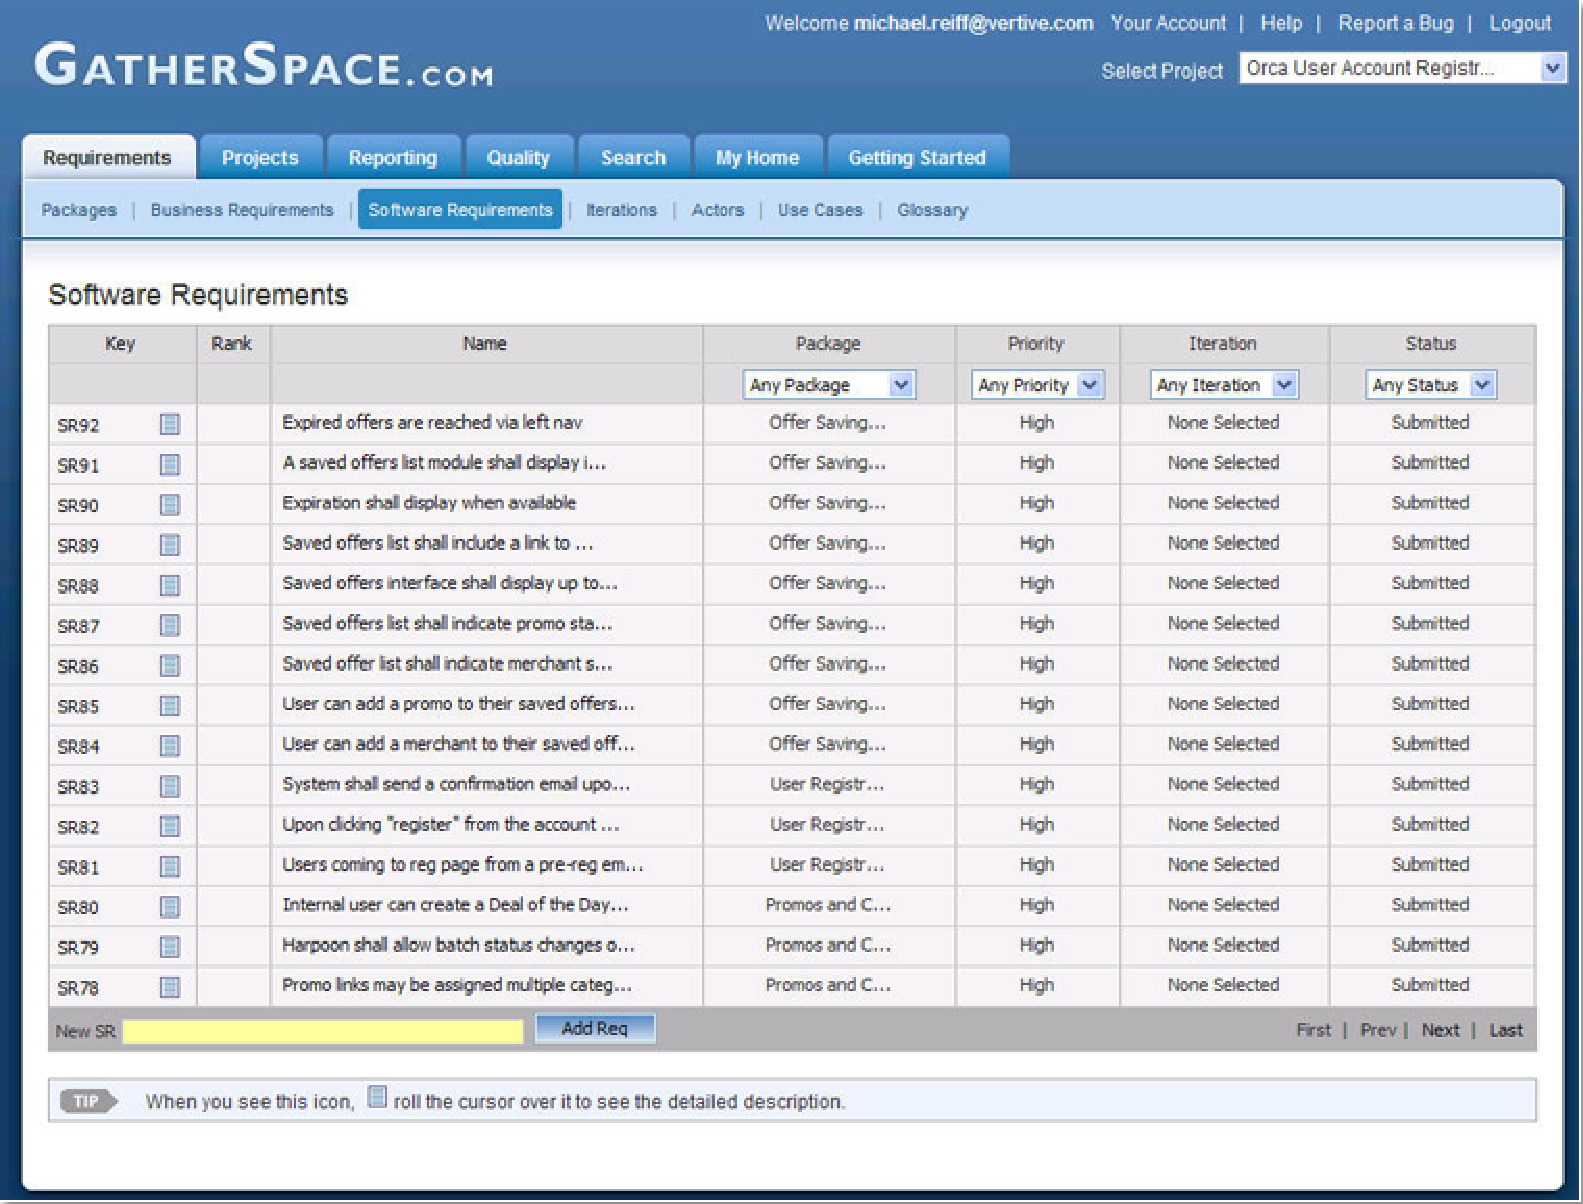
\includegraphics[width=1.0\textwidth]{img/gatherspace_2.pdf}
        \caption{Gatherspace.com - software requirements}
        \label{fig:gatherspace_2}
      \end{figure*}

      \begin{figure*}[t]
        \centering
        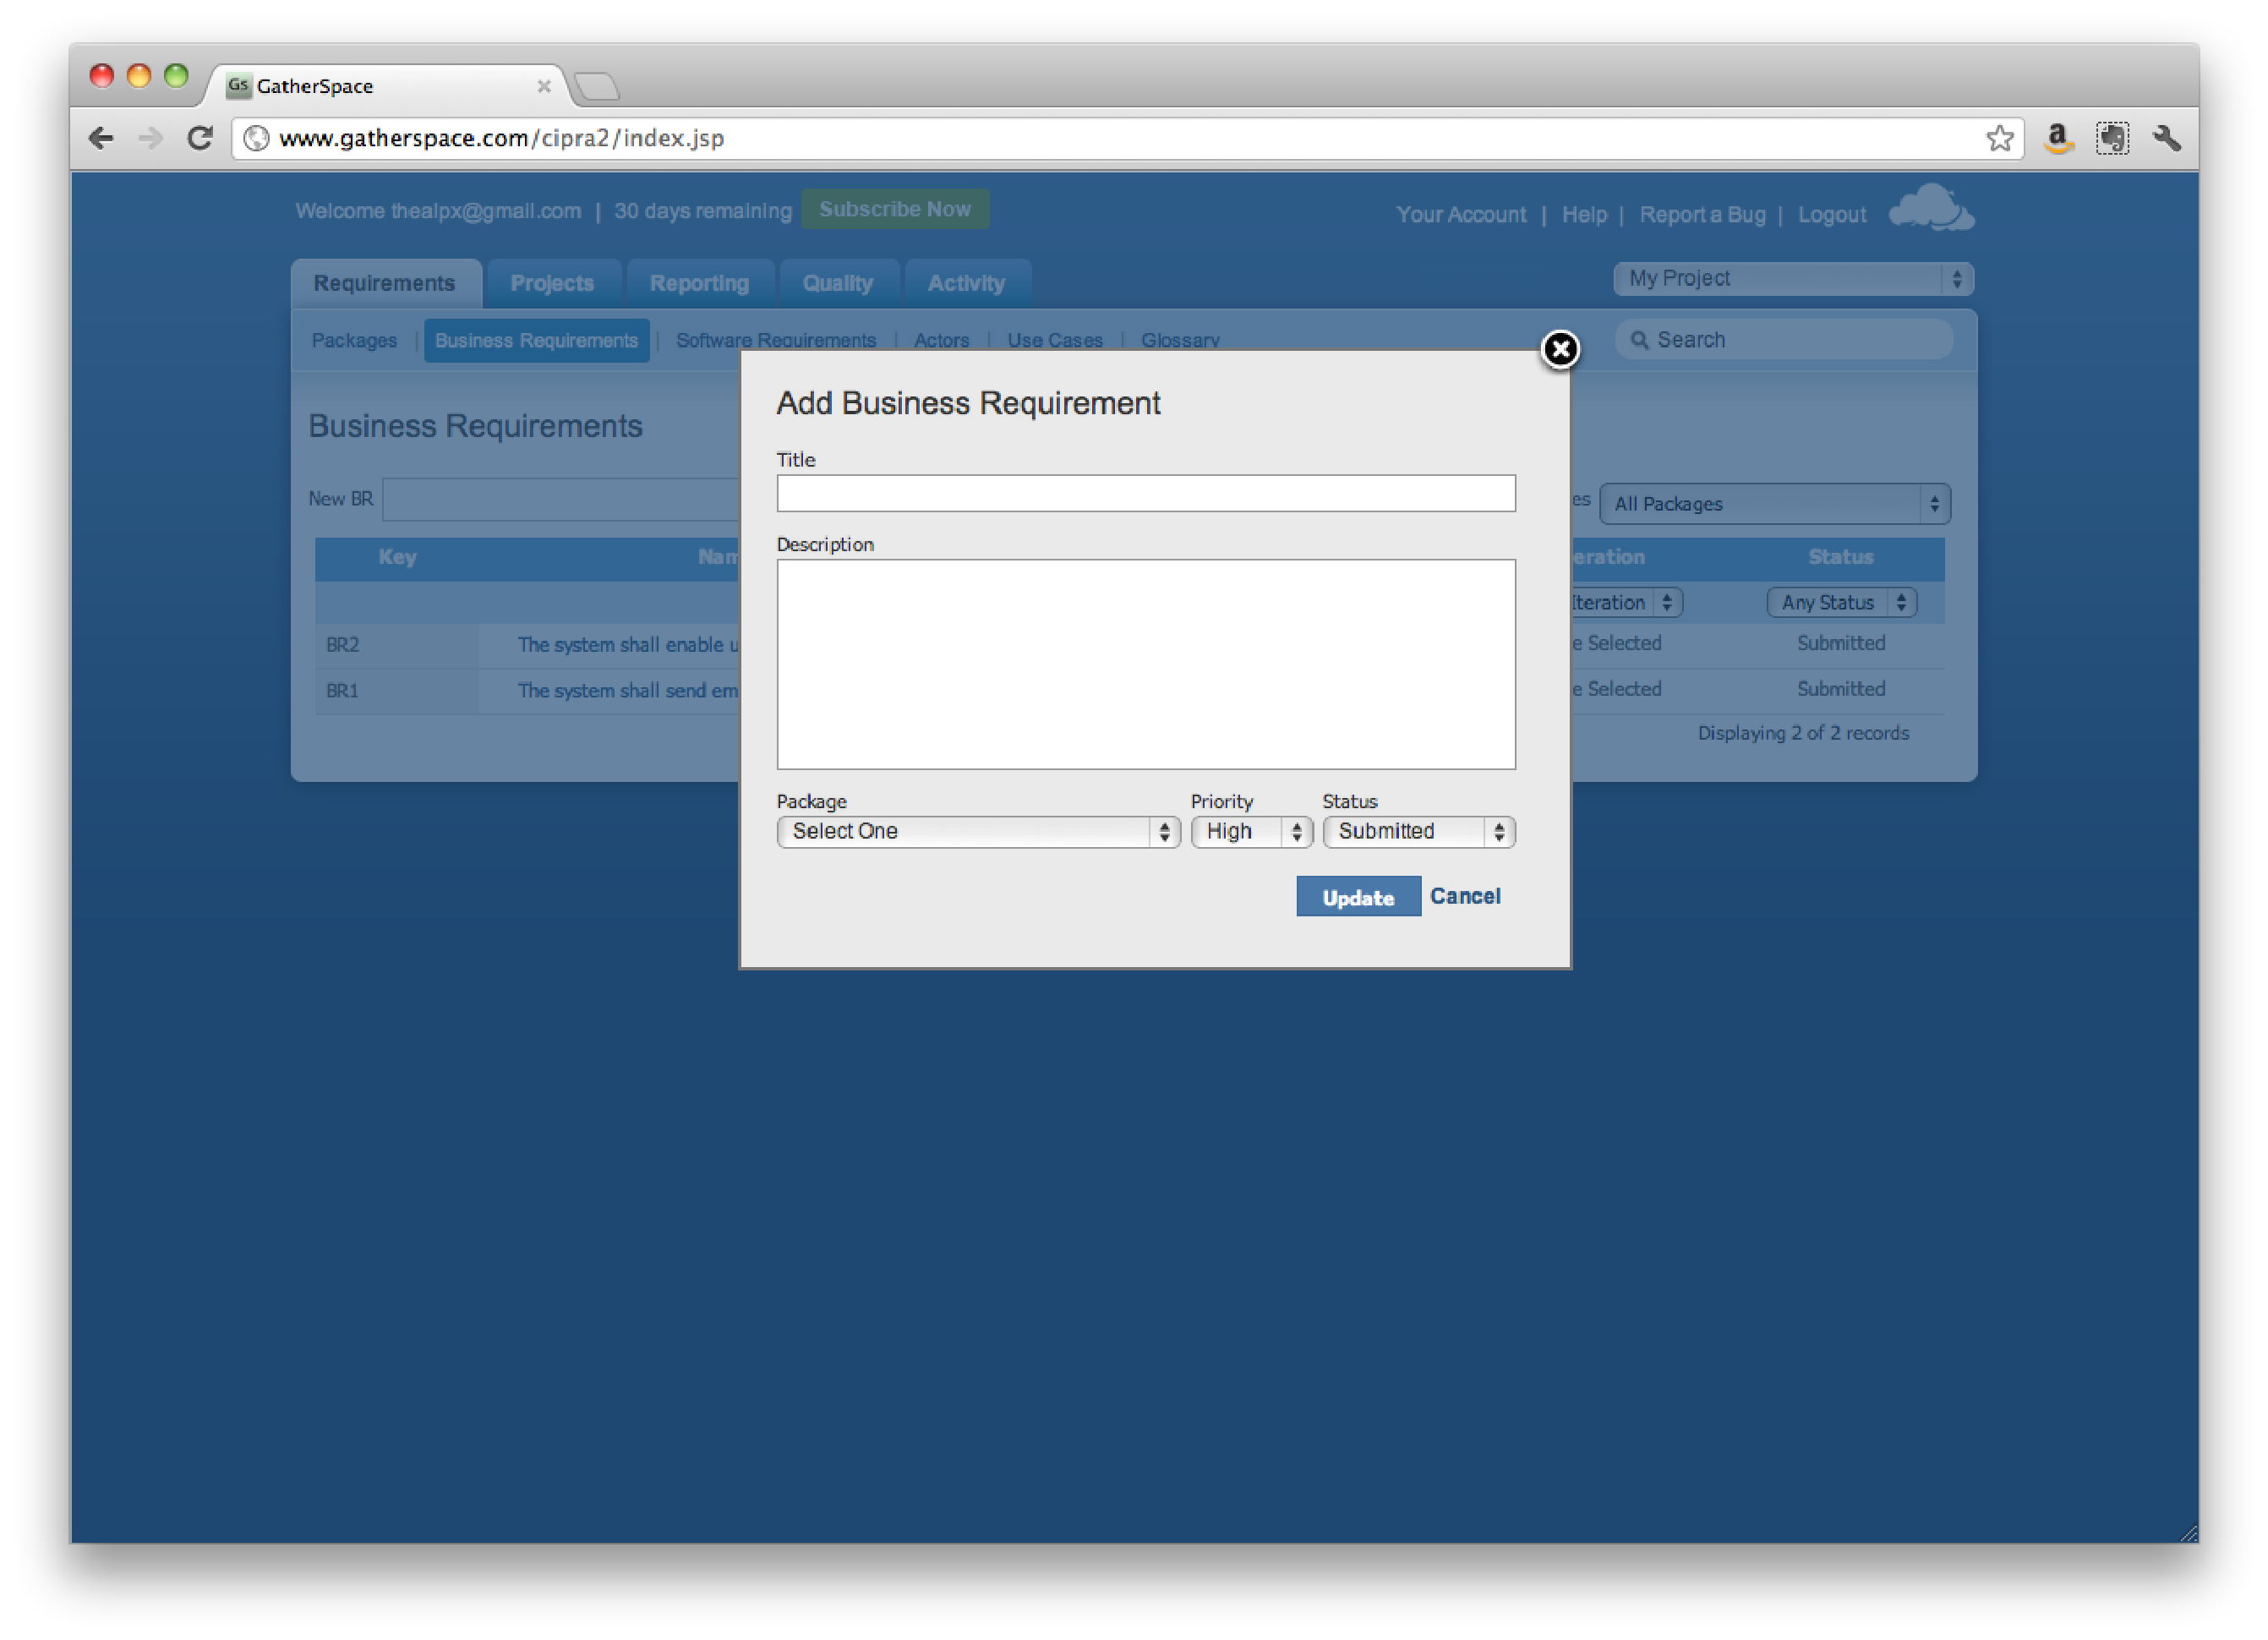
\includegraphics[width=1.0\textwidth]{img/gatherspace_5.pdf}
        \caption{Gatherspace.com - dodawanie wymagania ze szczegółami}
        \label{fig:gatherspace_5}
      \end{figure*}

      \begin{figure*}[t]
        \centering
        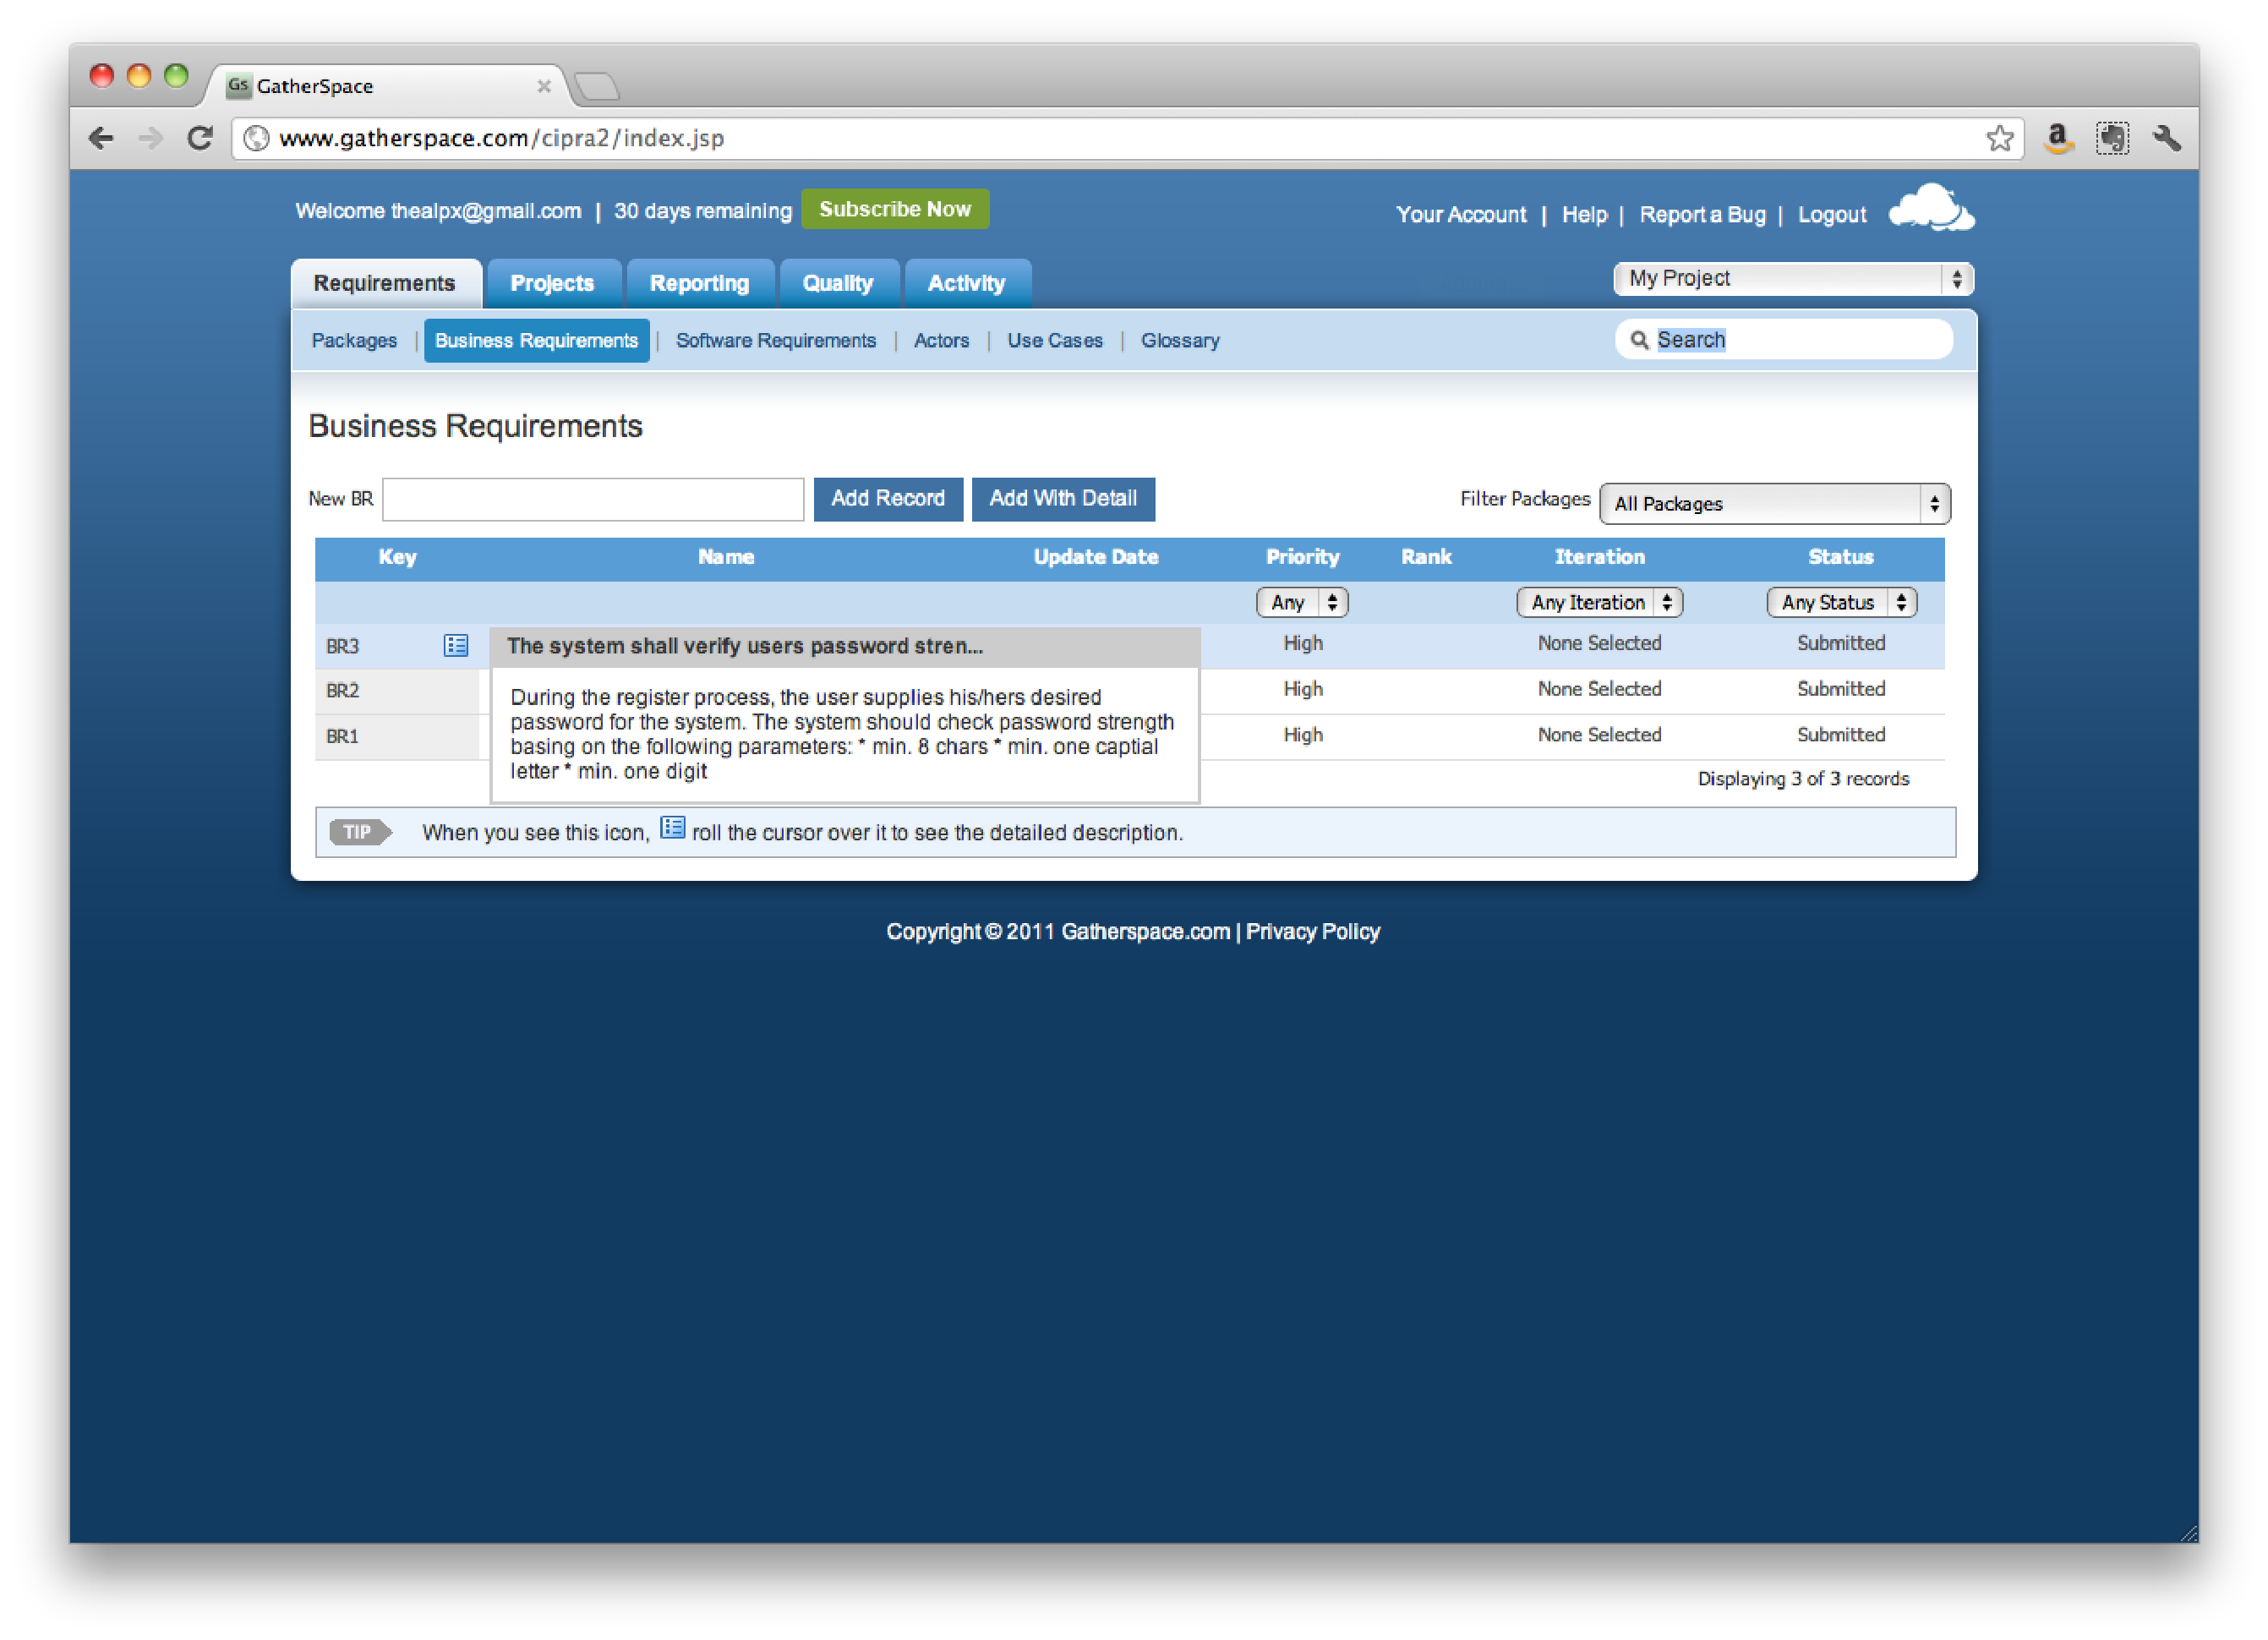
\includegraphics[width=1.0\textwidth]{img/gatherspace_6.pdf}
        \caption{Gatherspace.com - tooltip ze szczegółami wymagania}
        \label{fig:gatherspace_6}
      \end{figure*}

      \begin{figure*}[t]
        \centering
        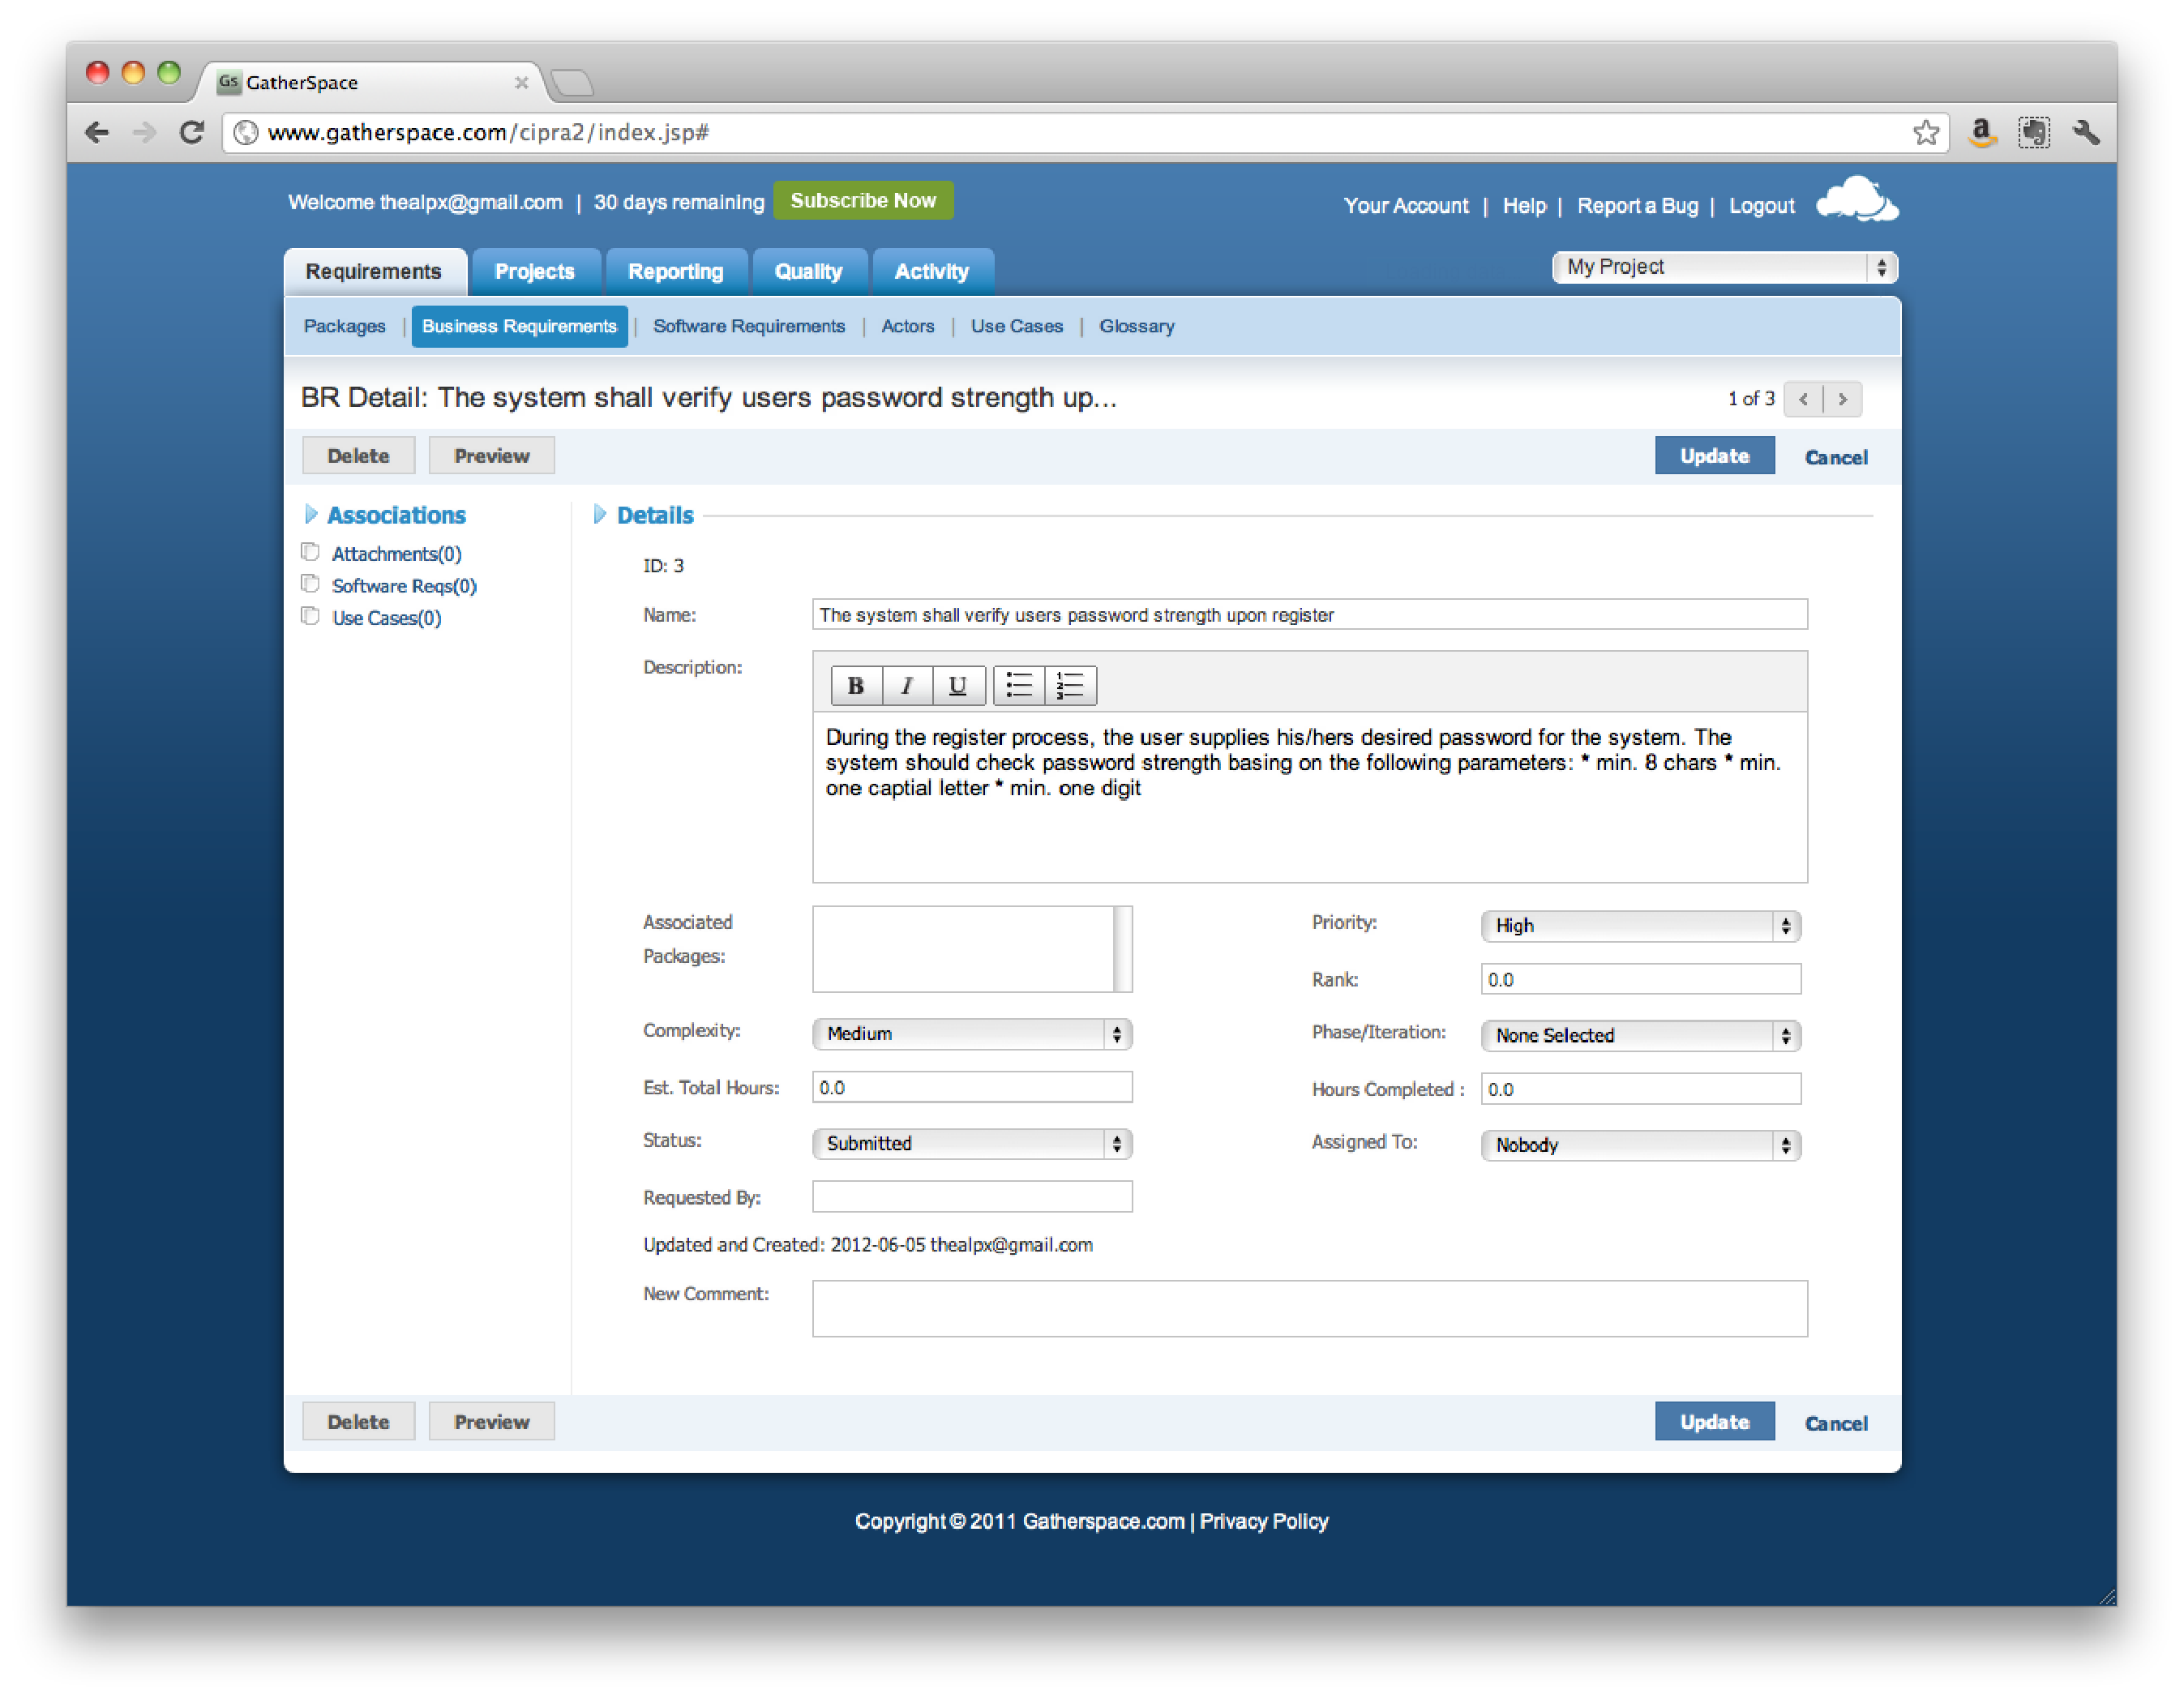
\includegraphics[width=1.0\textwidth]{img/gatherspace_7.pdf}
        \caption{Gatherspace.com - widok szczegółów wymagania}
        \label{fig:gatherspace_7}
      \end{figure*}

      \begin{figure*}[t]
        \centering
        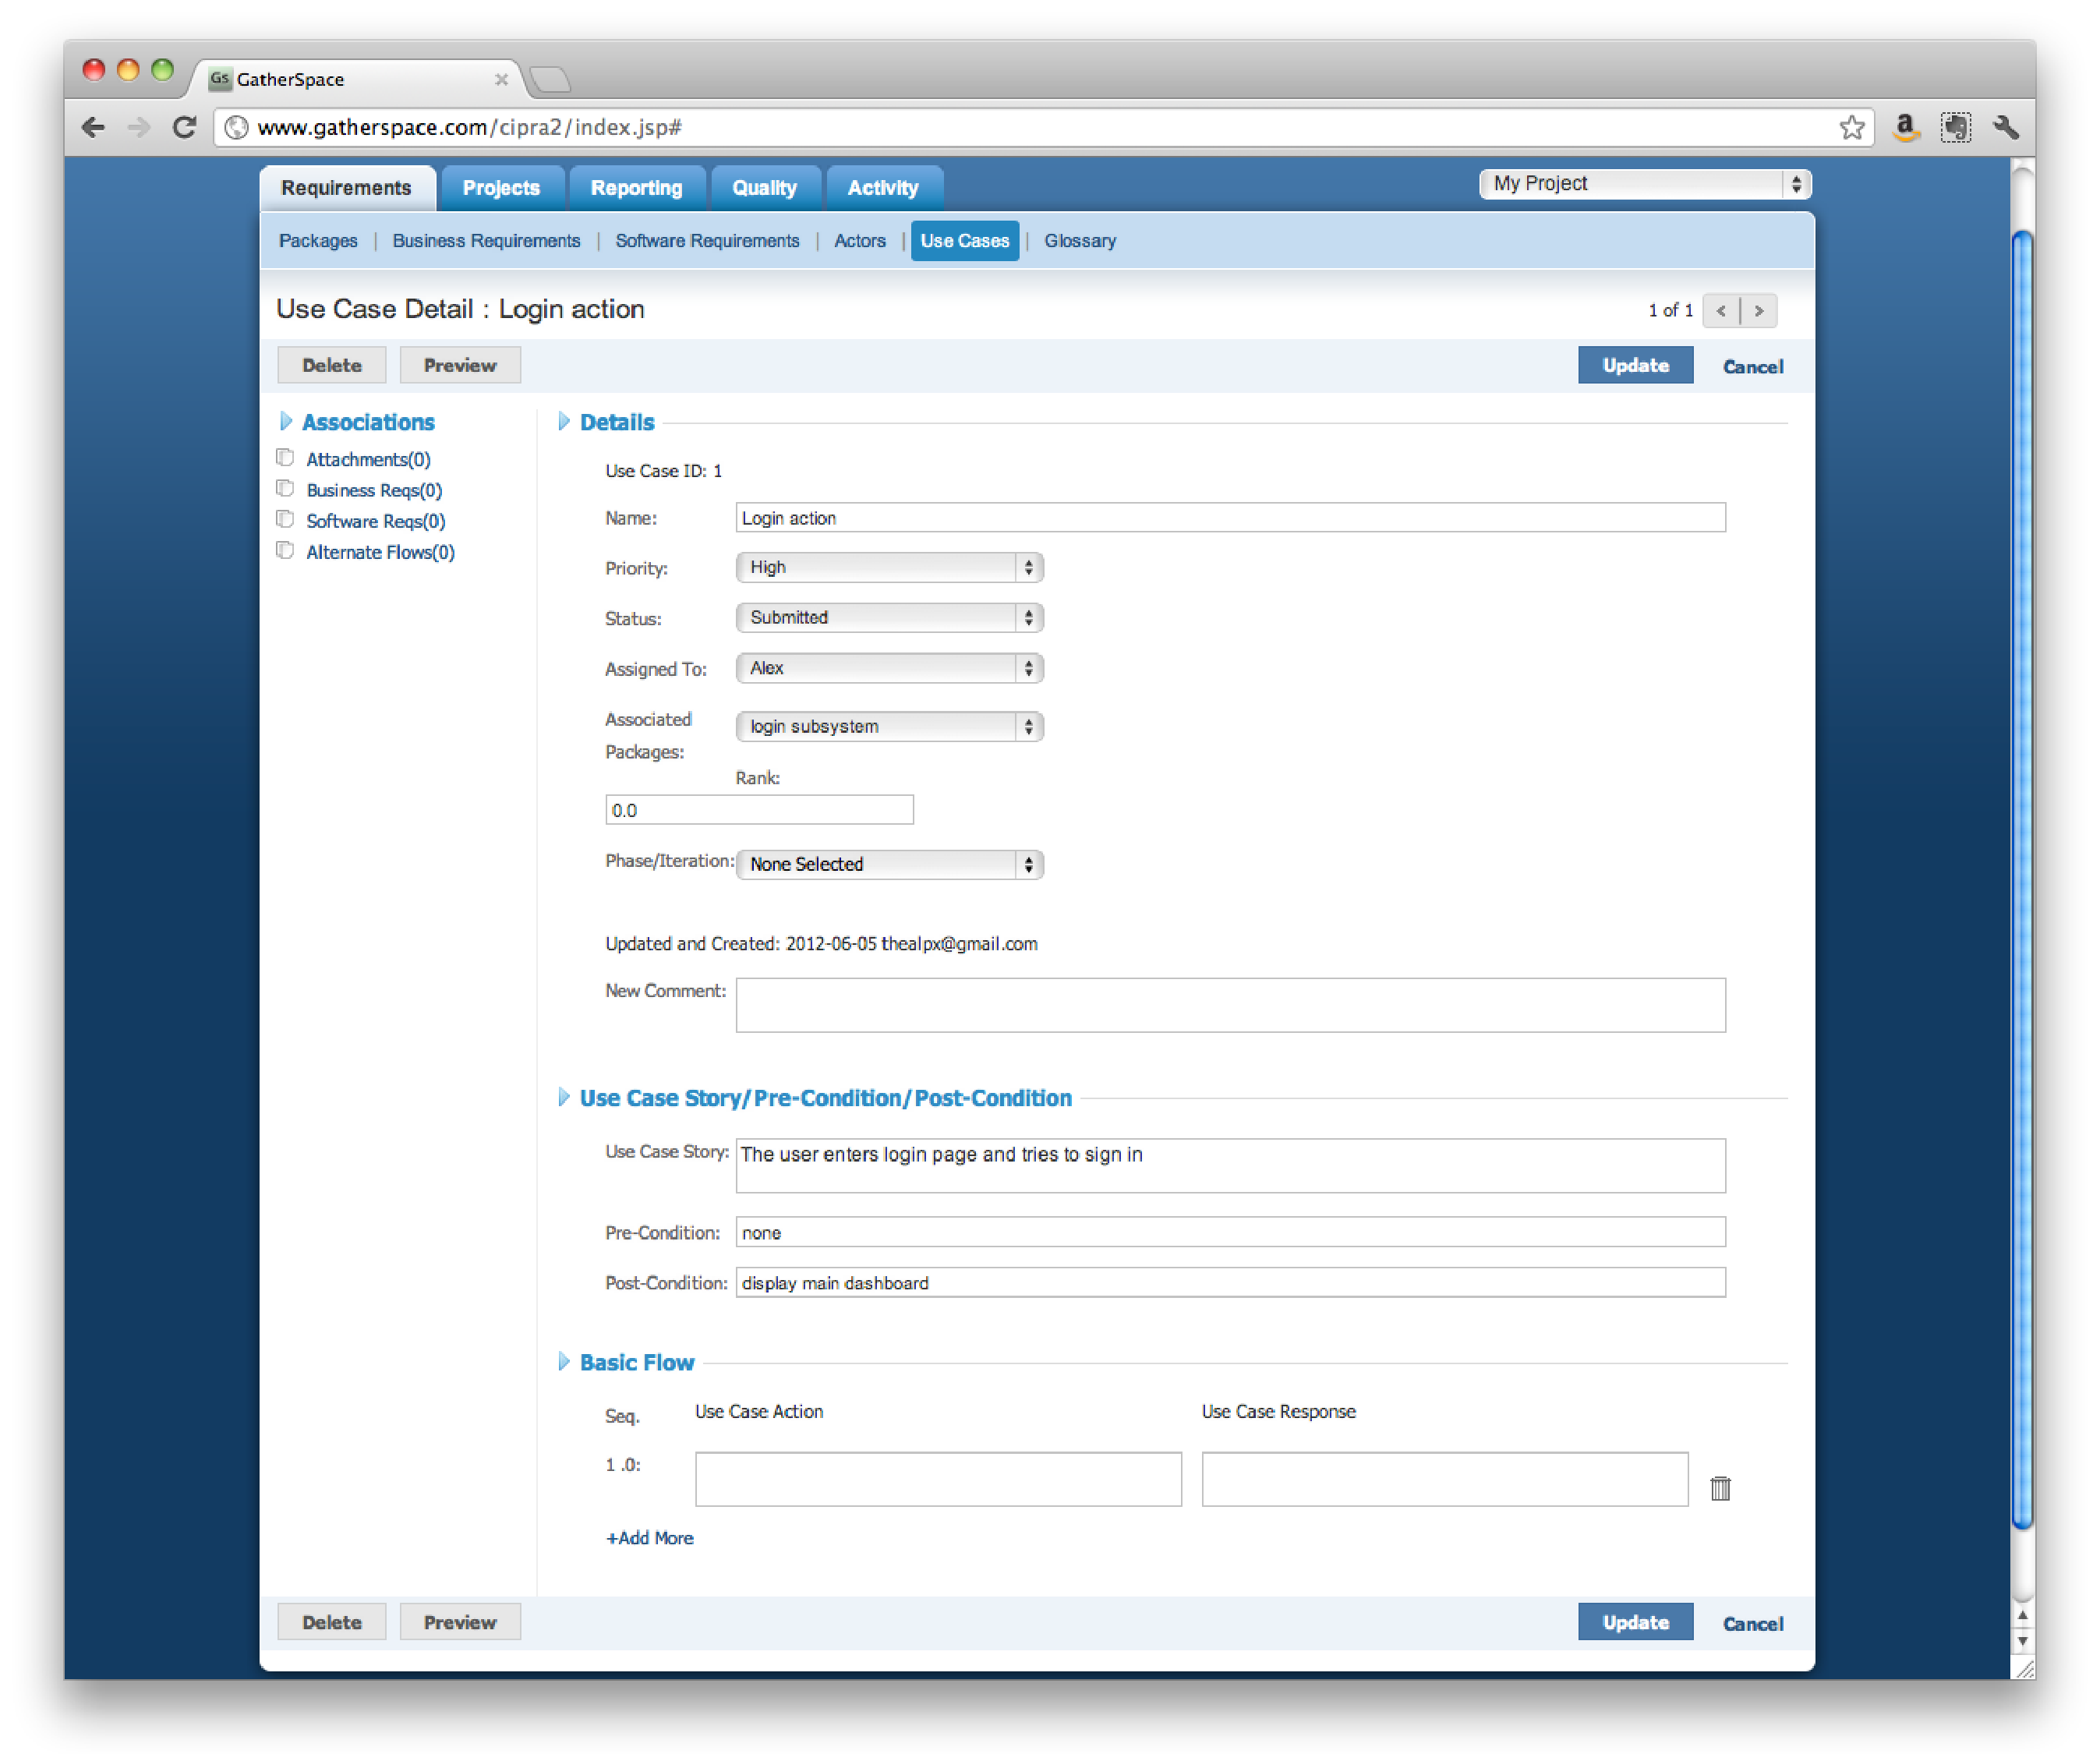
\includegraphics[width=1.0\textwidth]{img/gatherspace_8.pdf}
        \caption{Gatherspace.com - widok szczegółów wymagania}
        \label{fig:gatherspace_8}
      \end{figure*}

      \begin{figure*}[t]
        \centering
        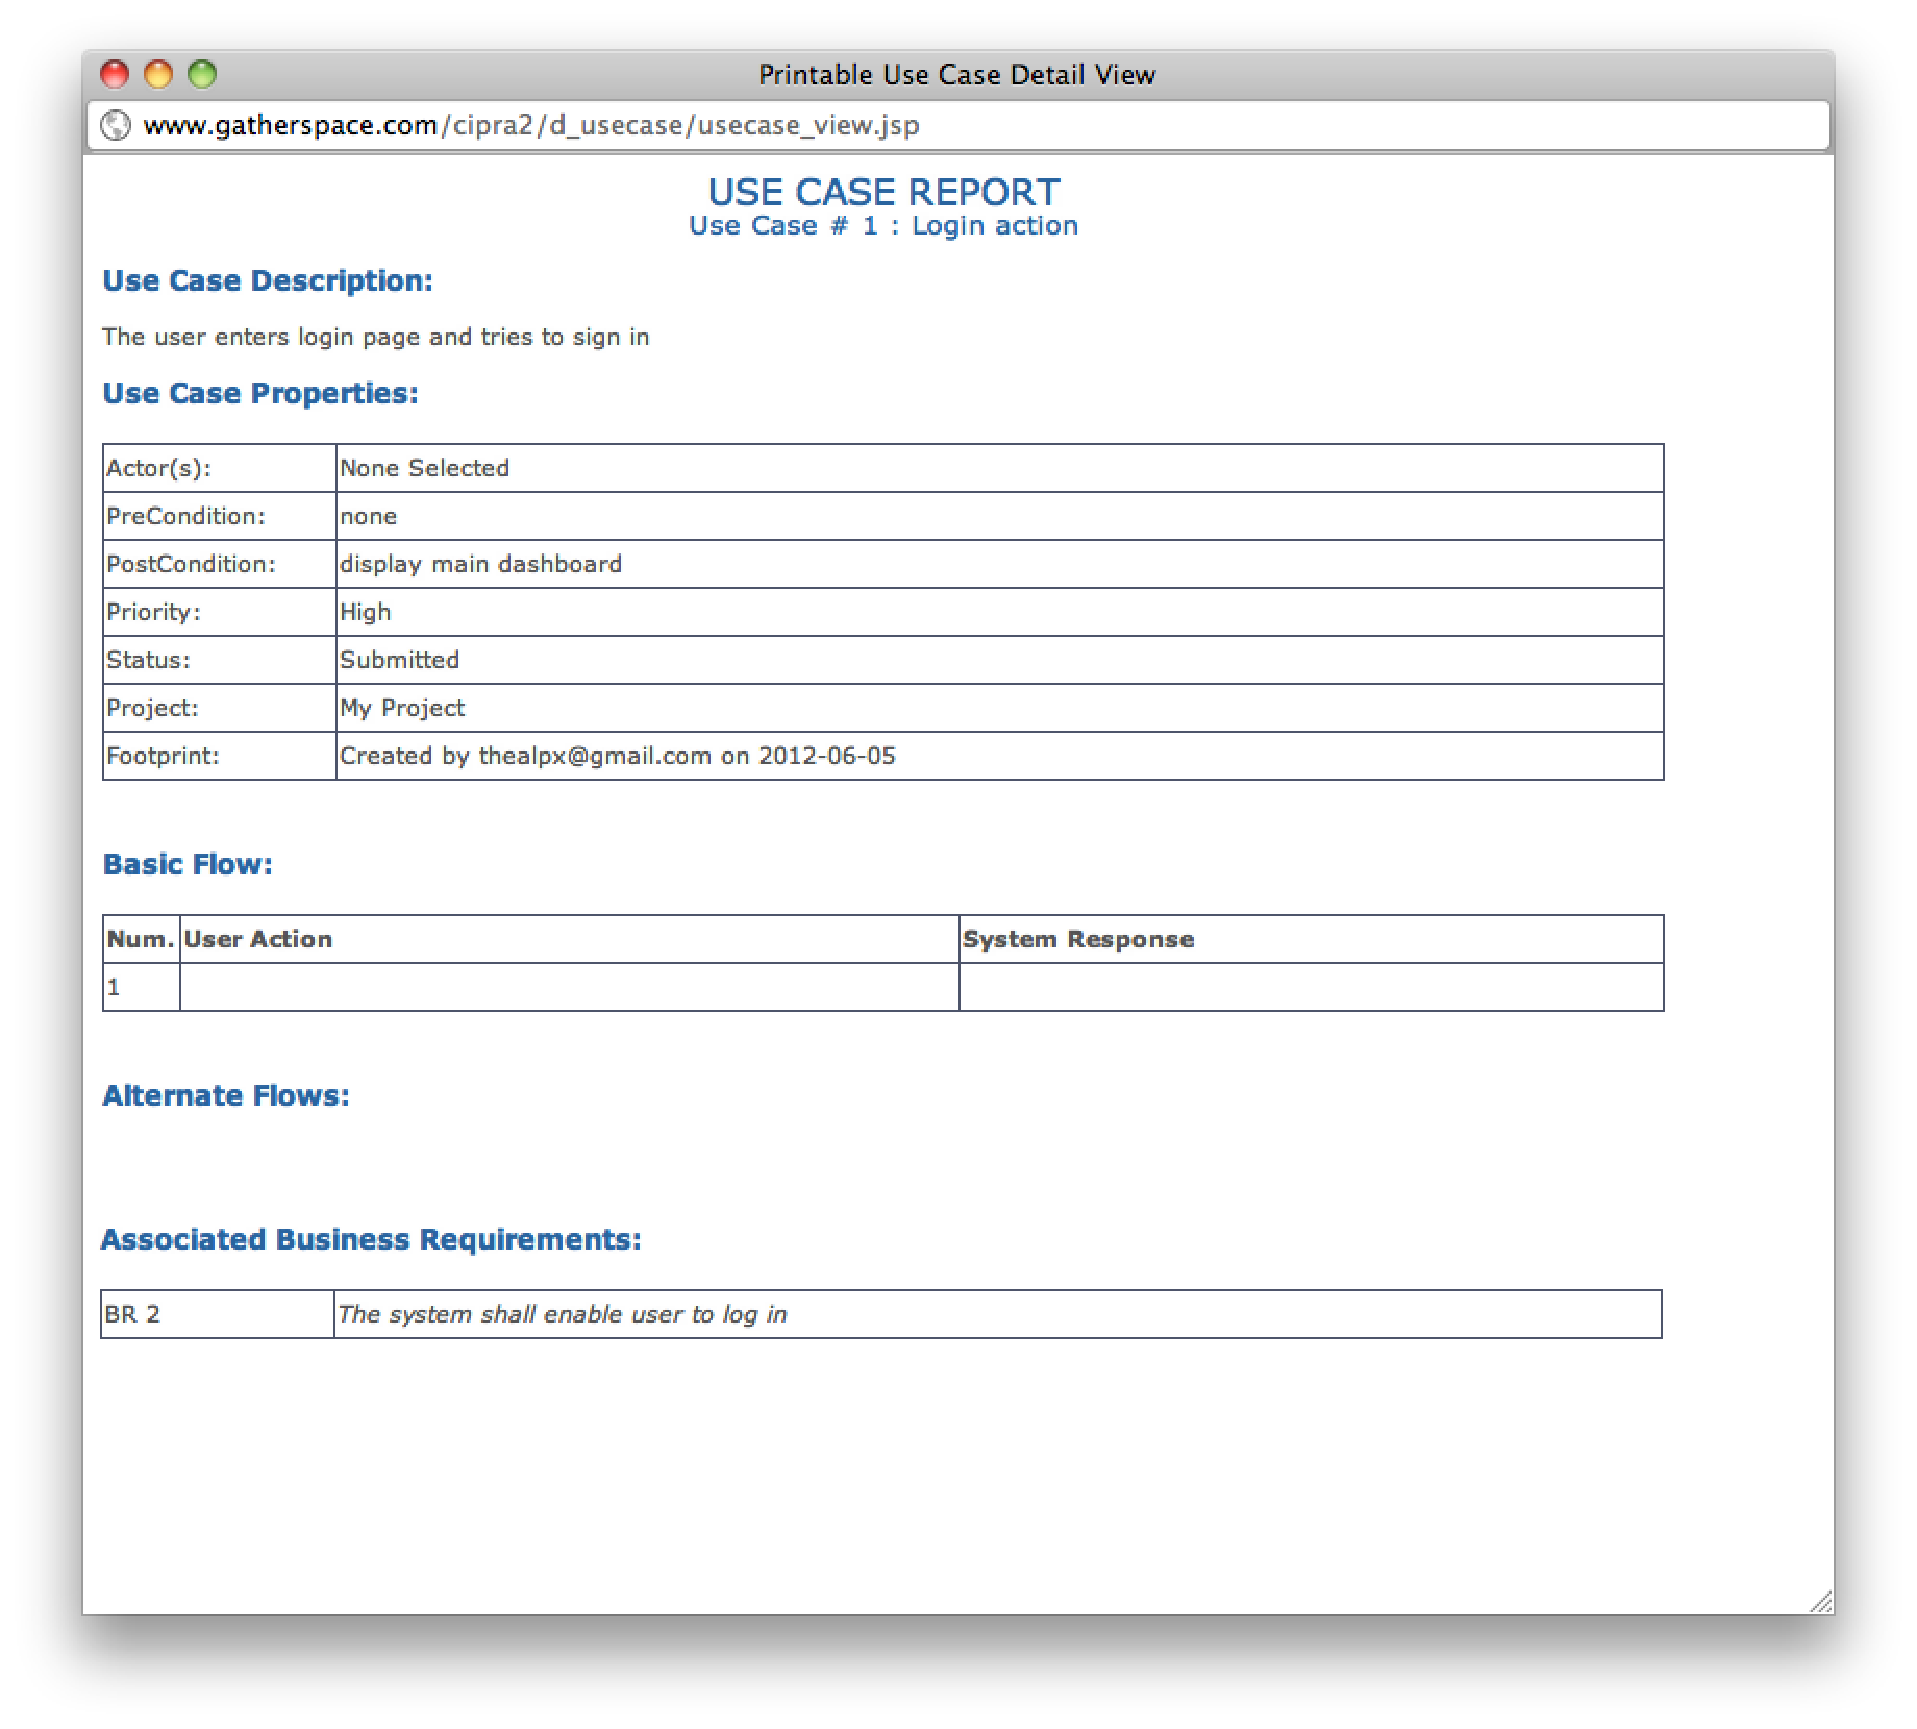
\includegraphics[width=1.0\textwidth]{img/gatherspace_9.pdf}
        \caption{Gatherspace.com - wymaganie przygotowane do druku}
        \label{fig:gatherspace_9}
      \end{figure*}

      \begin{figure*}[t]
        \centering
        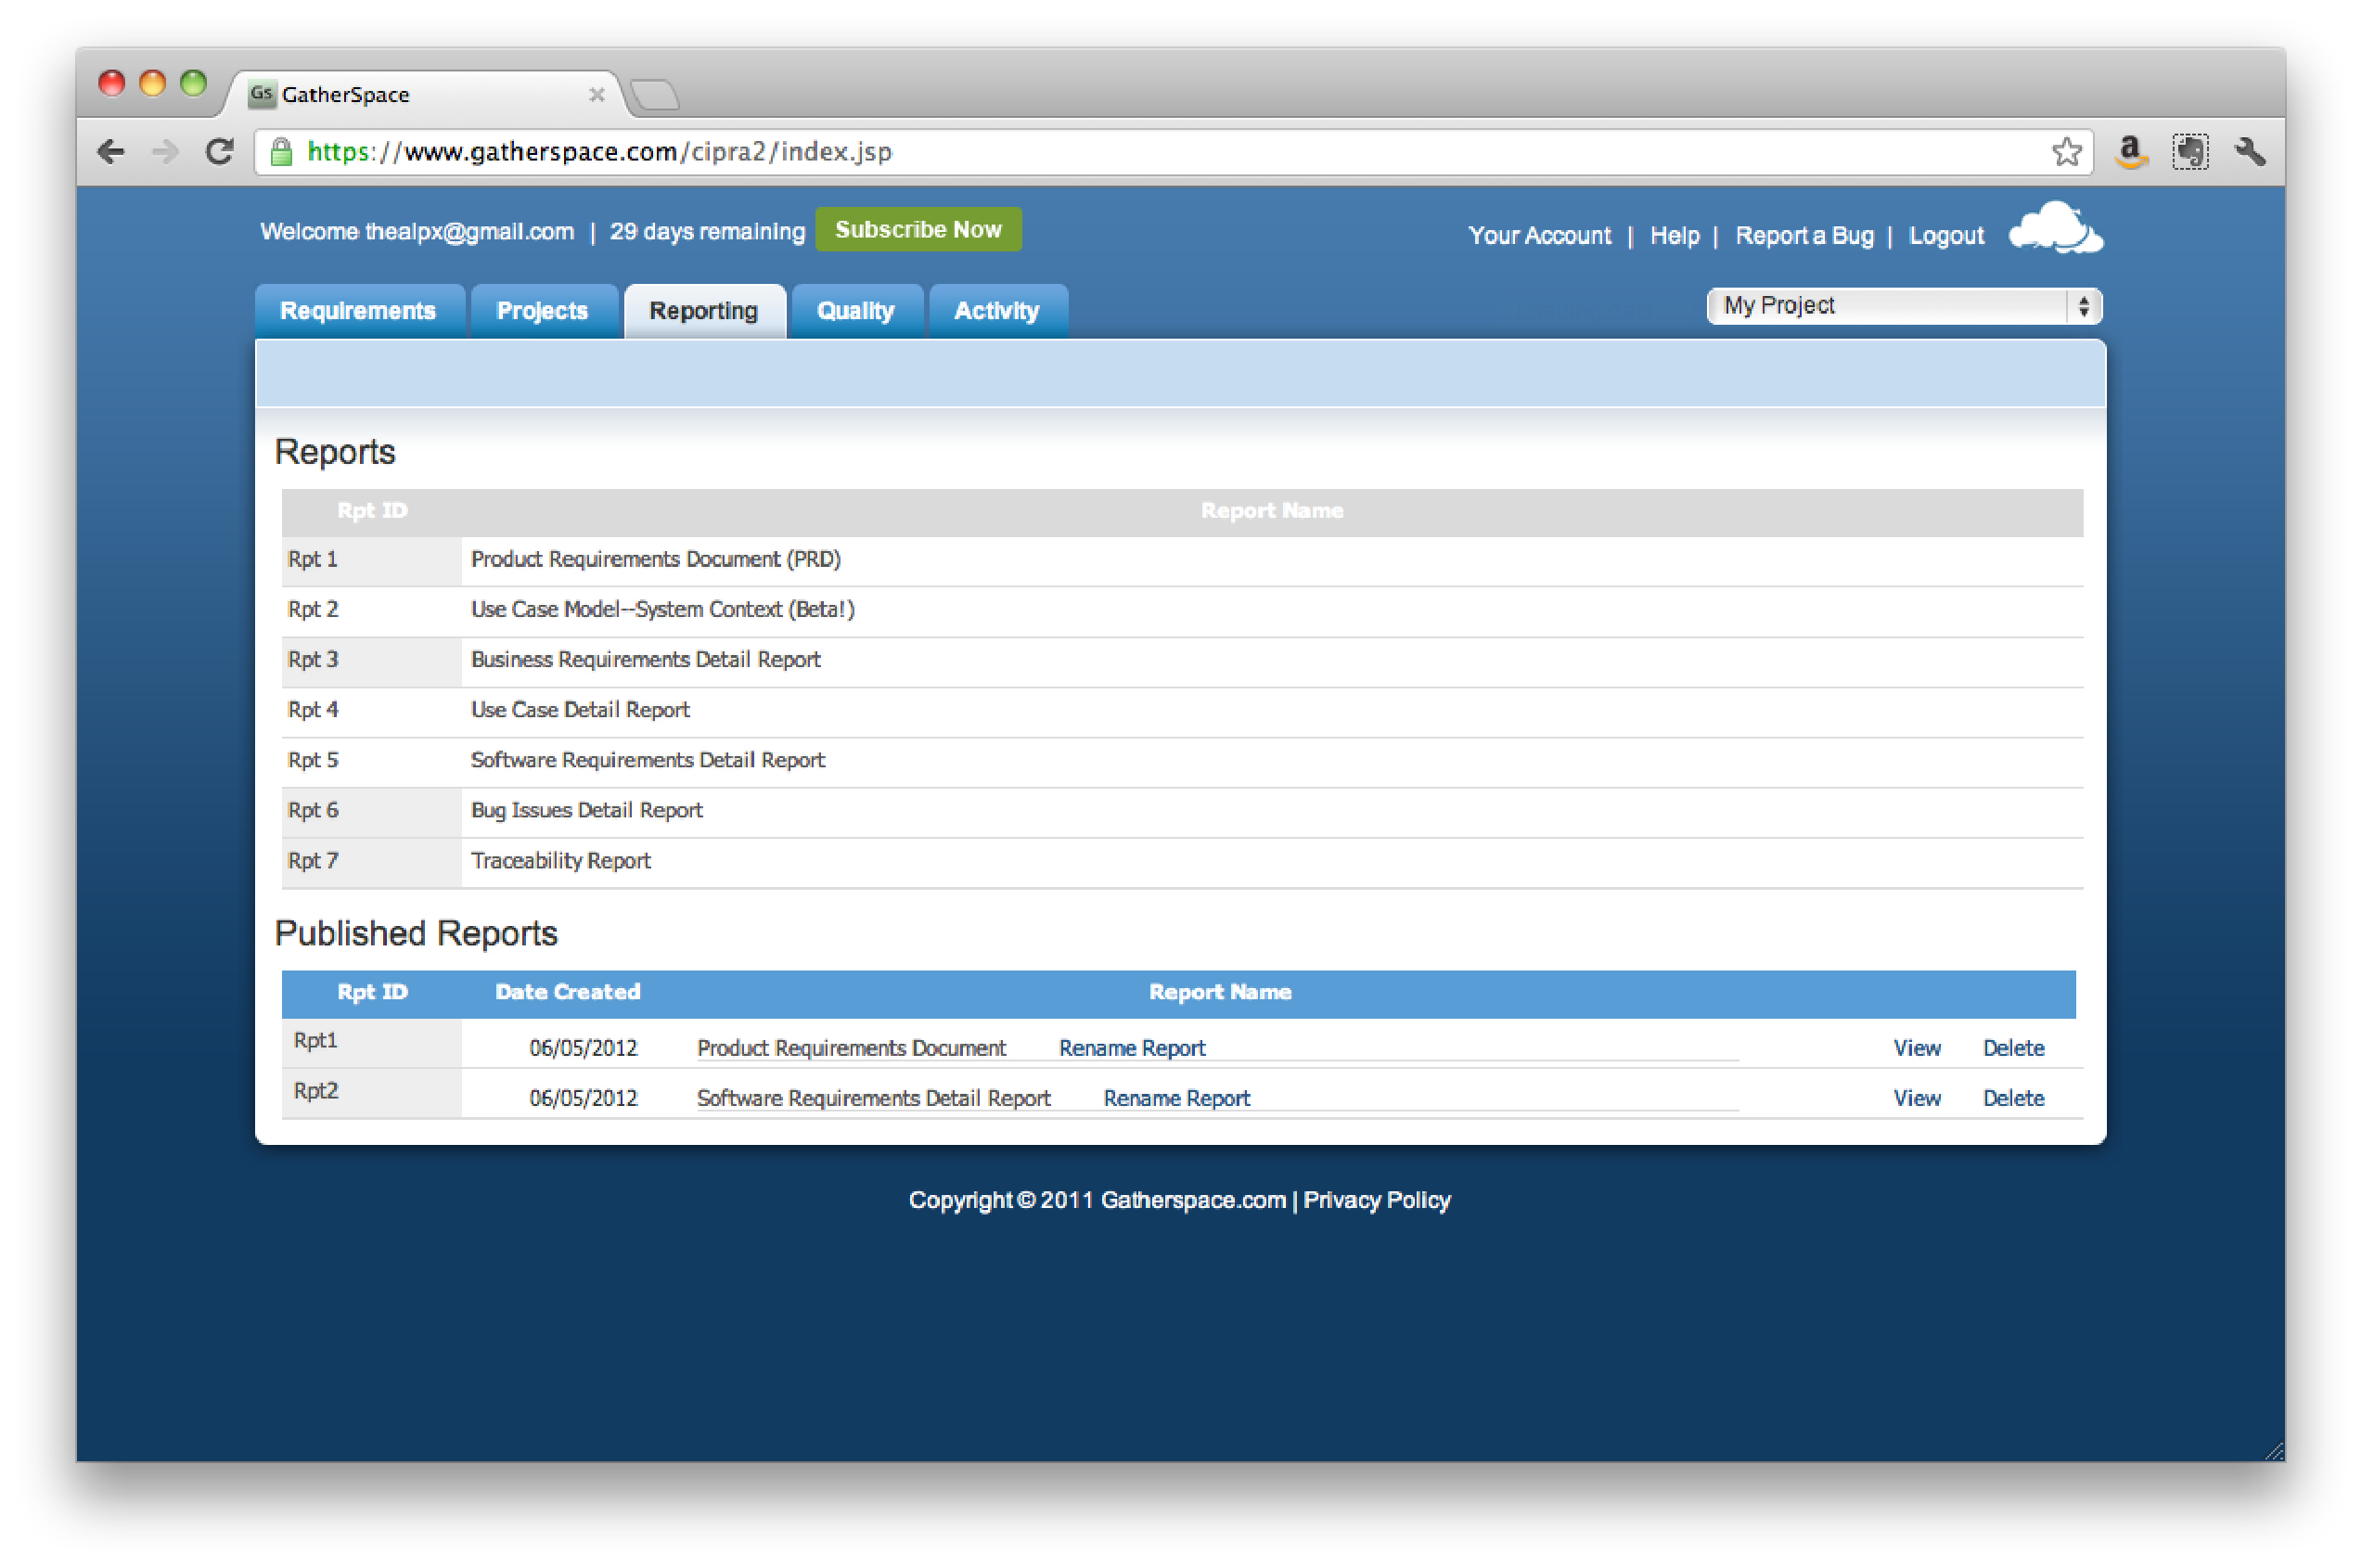
\includegraphics[width=1.0\textwidth]{img/gatherspace_11.pdf}
        \caption{Gatherspace.com - dostępne raporty}
        \label{fig:gatherspace_11}
      \end{figure*}

      \subsubsection{Gatherspace}
        Gatherspace dzieli wymagania na biznesowe (business requirements) oraz funkcjonalne (software requirements). Dostępne są osobne widoki dla obu typów wymagań (rys. \ref{fig:gatherspace_1}, \ref{fig:gatherspace_2}). Wymagania można katalogować w definiowane przez użytkownika pakiety, podobnie jak pliki w katalogach, w systemach operacyjnych. 


        Na rysunku \ref{fig:gatherspace_2} przedstawiono widok wymagań funkcjonalnych. Dodawanie wymagań przebiega w prosty sposób. Po wpisaniu tytułu wymagania i zatwierdzeniu pola formularza, element zostaje dodany do listy bez przeładowania strony.

        Wymaganie może zostać dodane na dwa sposoby - podając jedynie tytuł lub wybierając opcję ,,Add with detail''. Wówczas pojawia się ,,popup'' umożliwiający dodanie zarówno treści jak i opisu wymagania (patrz rys. \ref{fig:gatherspace_5}).

        Wymaganie posiadające opis, zaopatrzone jest w specjalną ikonkę po lewej stronie. Użytkownik wskazujący w to miejsce myszką może podejrzeć treść wymagania, bez konieczności otwierania jego szczegółów. Jest to dość przydatna funkcjonalność, pozwalająca szybko zapoznać się pobieżnie z danym wymaganiem. Rysunek \ref{fig:gatherspace_6} zawiera zrzut ekraniu prezentujący tę funkcjonalność. 
        
        Widok szczegółów wymagania jest dość prosty i przejrzysty (rys. \ref{fig:gatherspace_7}). Do dyspozycji użytkownika jest formularz zawierający pola z parametrami wymagania, takimi jak m.in.: priorytet, status, poziom złożoności, pakiet do którego należy, przez kogo wymaganie zostało dodane oraz kto lub co jest źródłem wymagania.

        Dodawanie przypadków użycia jest wydzielone do osobnego widoku i funkcjonuje jako osobny zestaw formularzy (rys. \ref{fig:gatherspace_8}). 

        Istnieje możliwość łączenia przypadków użycia z wymaganiami poprzez wskazanie konkretnego wymagania w osobnym widoku, jednak system nie umożliwia łączenia tych artefaktów z poziomu edytora graficznego.

        Zarówno przypadki użycia jak i wymagania mogą zostać wyświetlone w formie przyjaznej do druku. Dla przykładu zamieszczono zrzut ekranu obrazujący jeden przypadek użycia przygotowany do druku na rys. \ref{fig:gatherspace_9}

        Dostępne w systemie raporty umożliwiają wyświetlenie i wydruk raportów dotyczących wymagań funkcjonalnych i niefunkcjonalnych, raport przypadków użycia oraz raport identyfikowalności (traceability report), umożliwiający przeanalizowanie związków pomiędzy wymaganiami a przypadkami użycia (patrz rysunek \ref{fig:gatherspace_11}). 

        \pagebreak

        Koszt zakupu licencji na oprogramowanie Gatherspace to minimum 19\$ za miesiąc użytkowania. Co ciekawe, istnieje możliwość zakupu wersji oprogramowania, które zostanie zainstalowane w infrastrukturze klienta. Jest to interesujące rozwiązanie dla klientów korporacyjnych, dla których przechowywanie danych na zewnętrznych serwerach jest wykluczone z powodów bezpieczeństwa (np. banki). Jednak koszt zakupu takiej licencji, jak można przeczytać na stronie gatherspace, to 4900\$ za instalację systemu. Dodatkowo firma żąda 295\$ miesięcznie za obsługę systemu. Biorąc pod uwagę zakres funkcjonalności oraz użyteczność systemu, są to ogromne kwoty, przewyższające, w ocenie autora, wartość dodaną wniesioną do organizacji wraz z wdrożeniem systemu Gatherspace.
         
        \begin{figure*}[t]
          \centering
          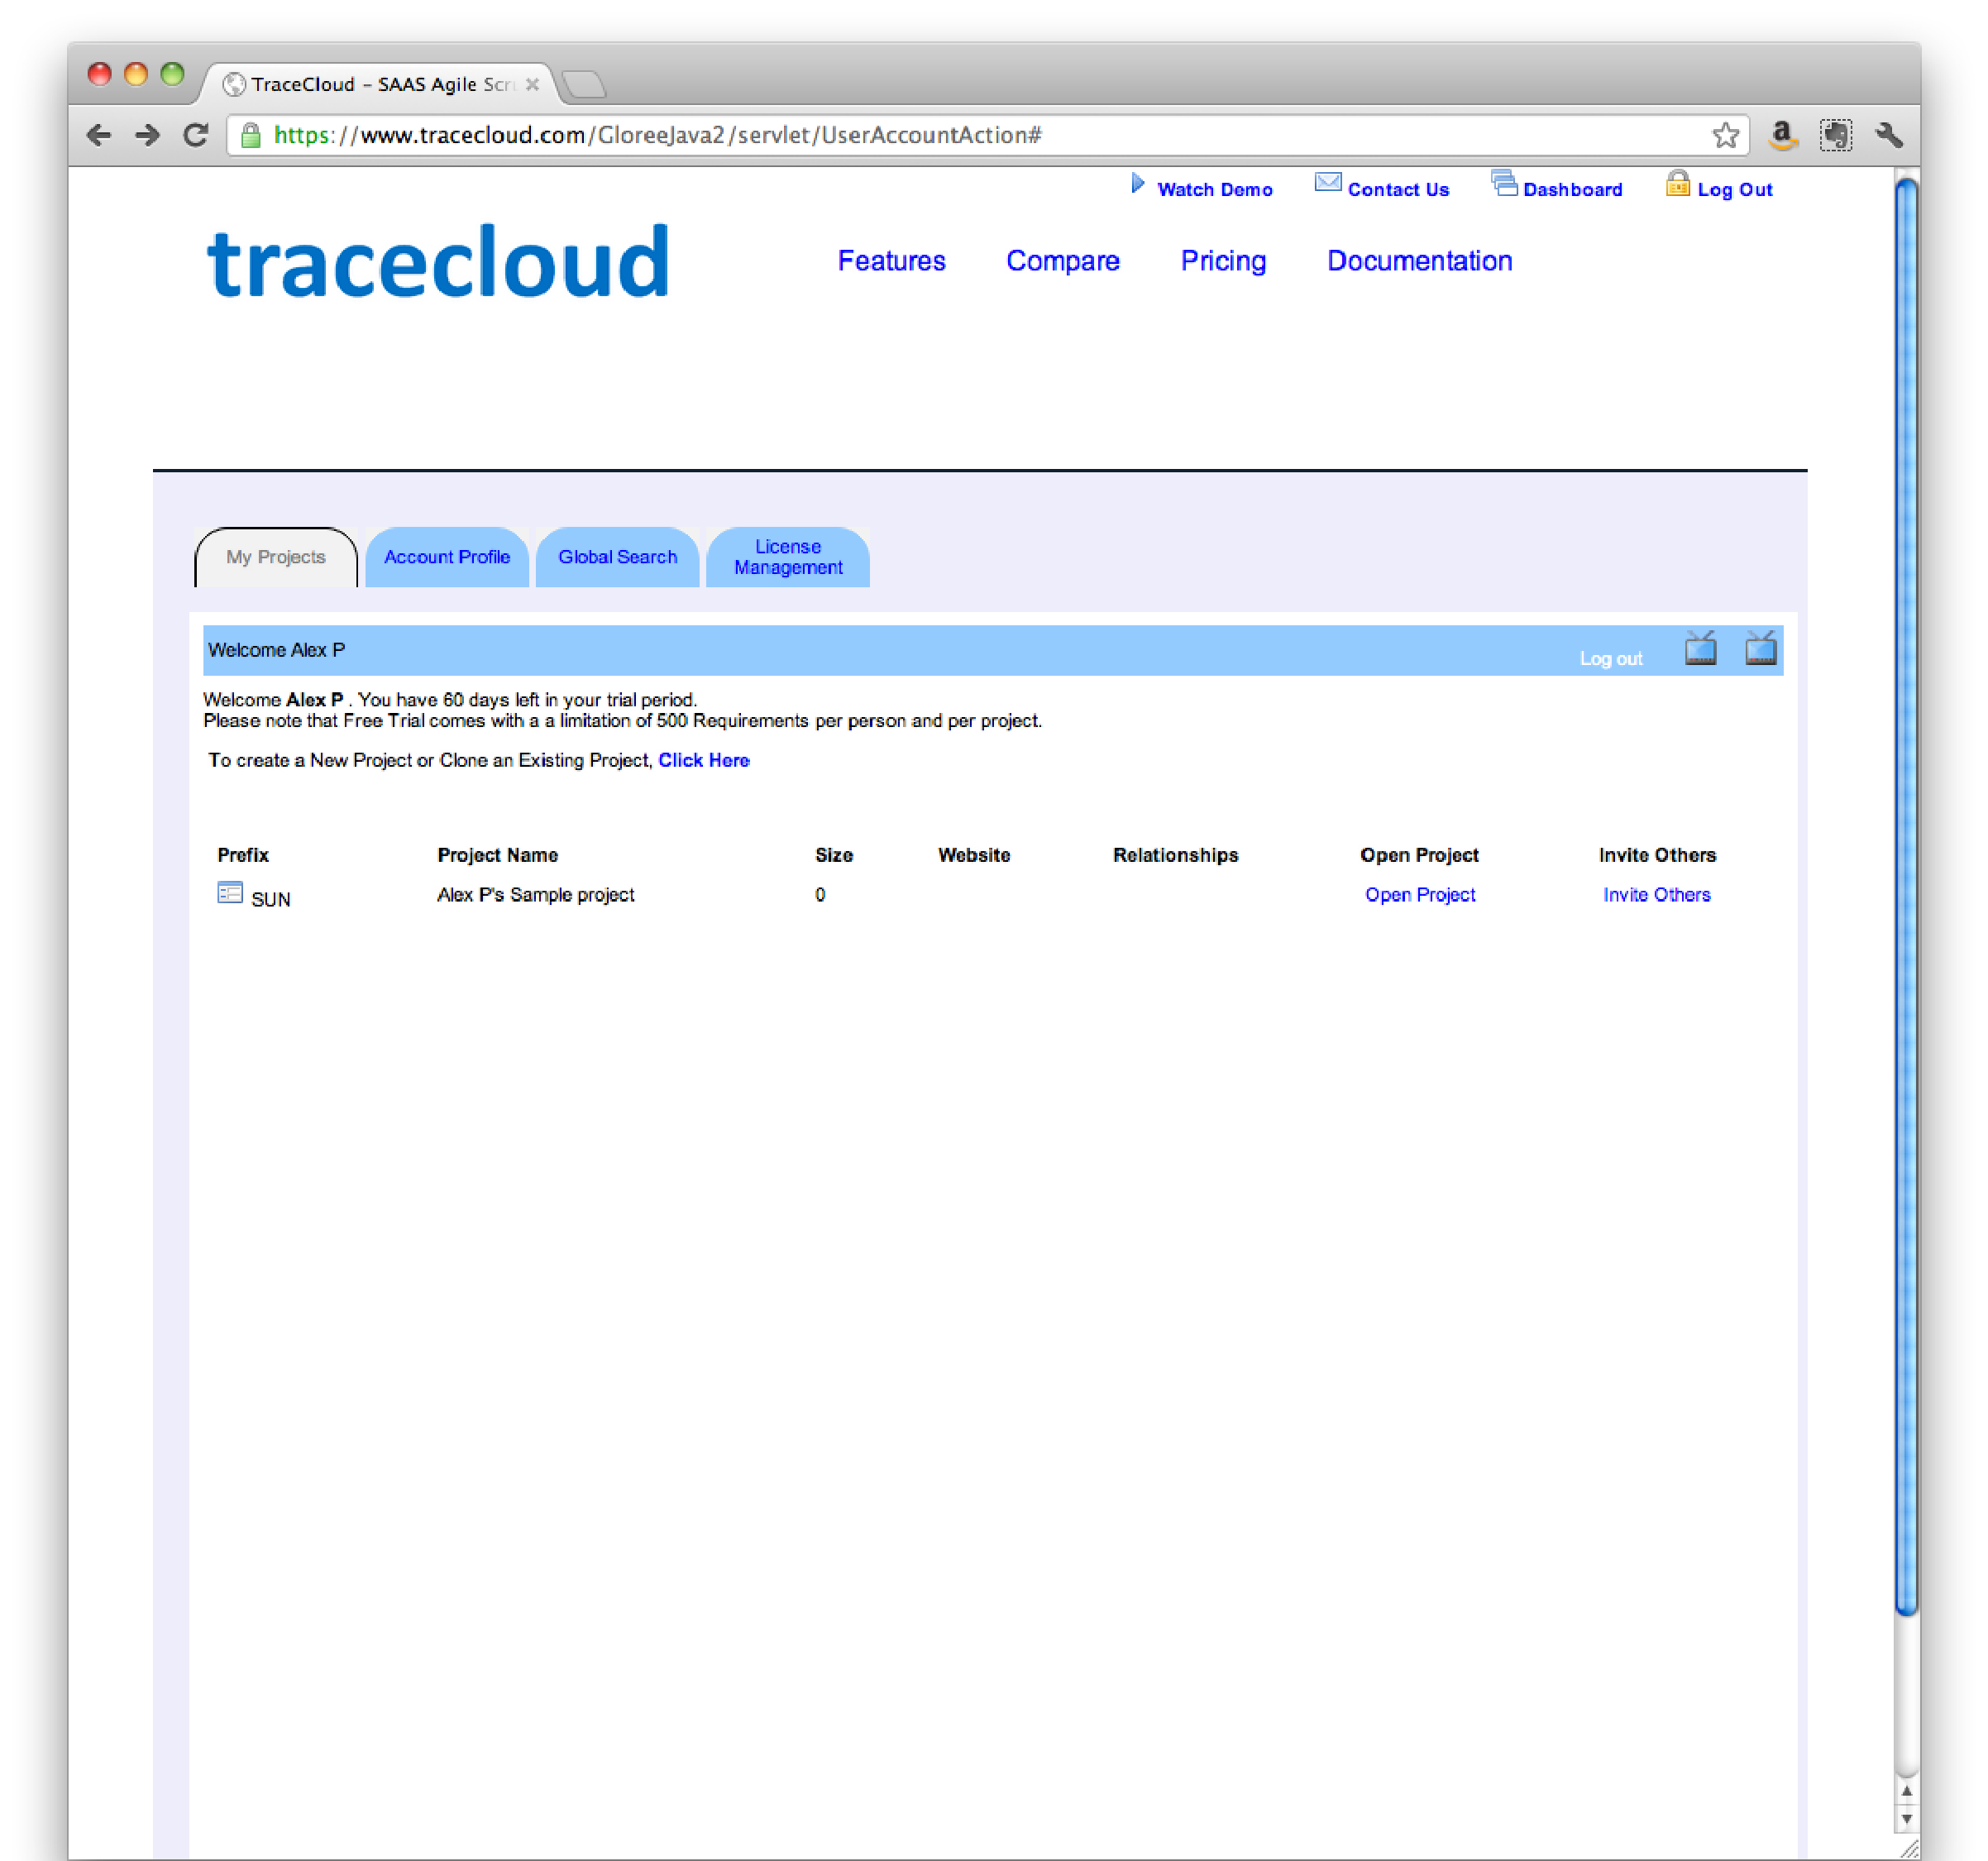
\includegraphics[width=1.0\textwidth]{img/tracecloud_1.pdf}
          \caption{Tracecloud - widok listy projektów}
          \label{fig:tracecloud_1}
        \end{figure*}

        \begin{figure*}[t]
          \centering
          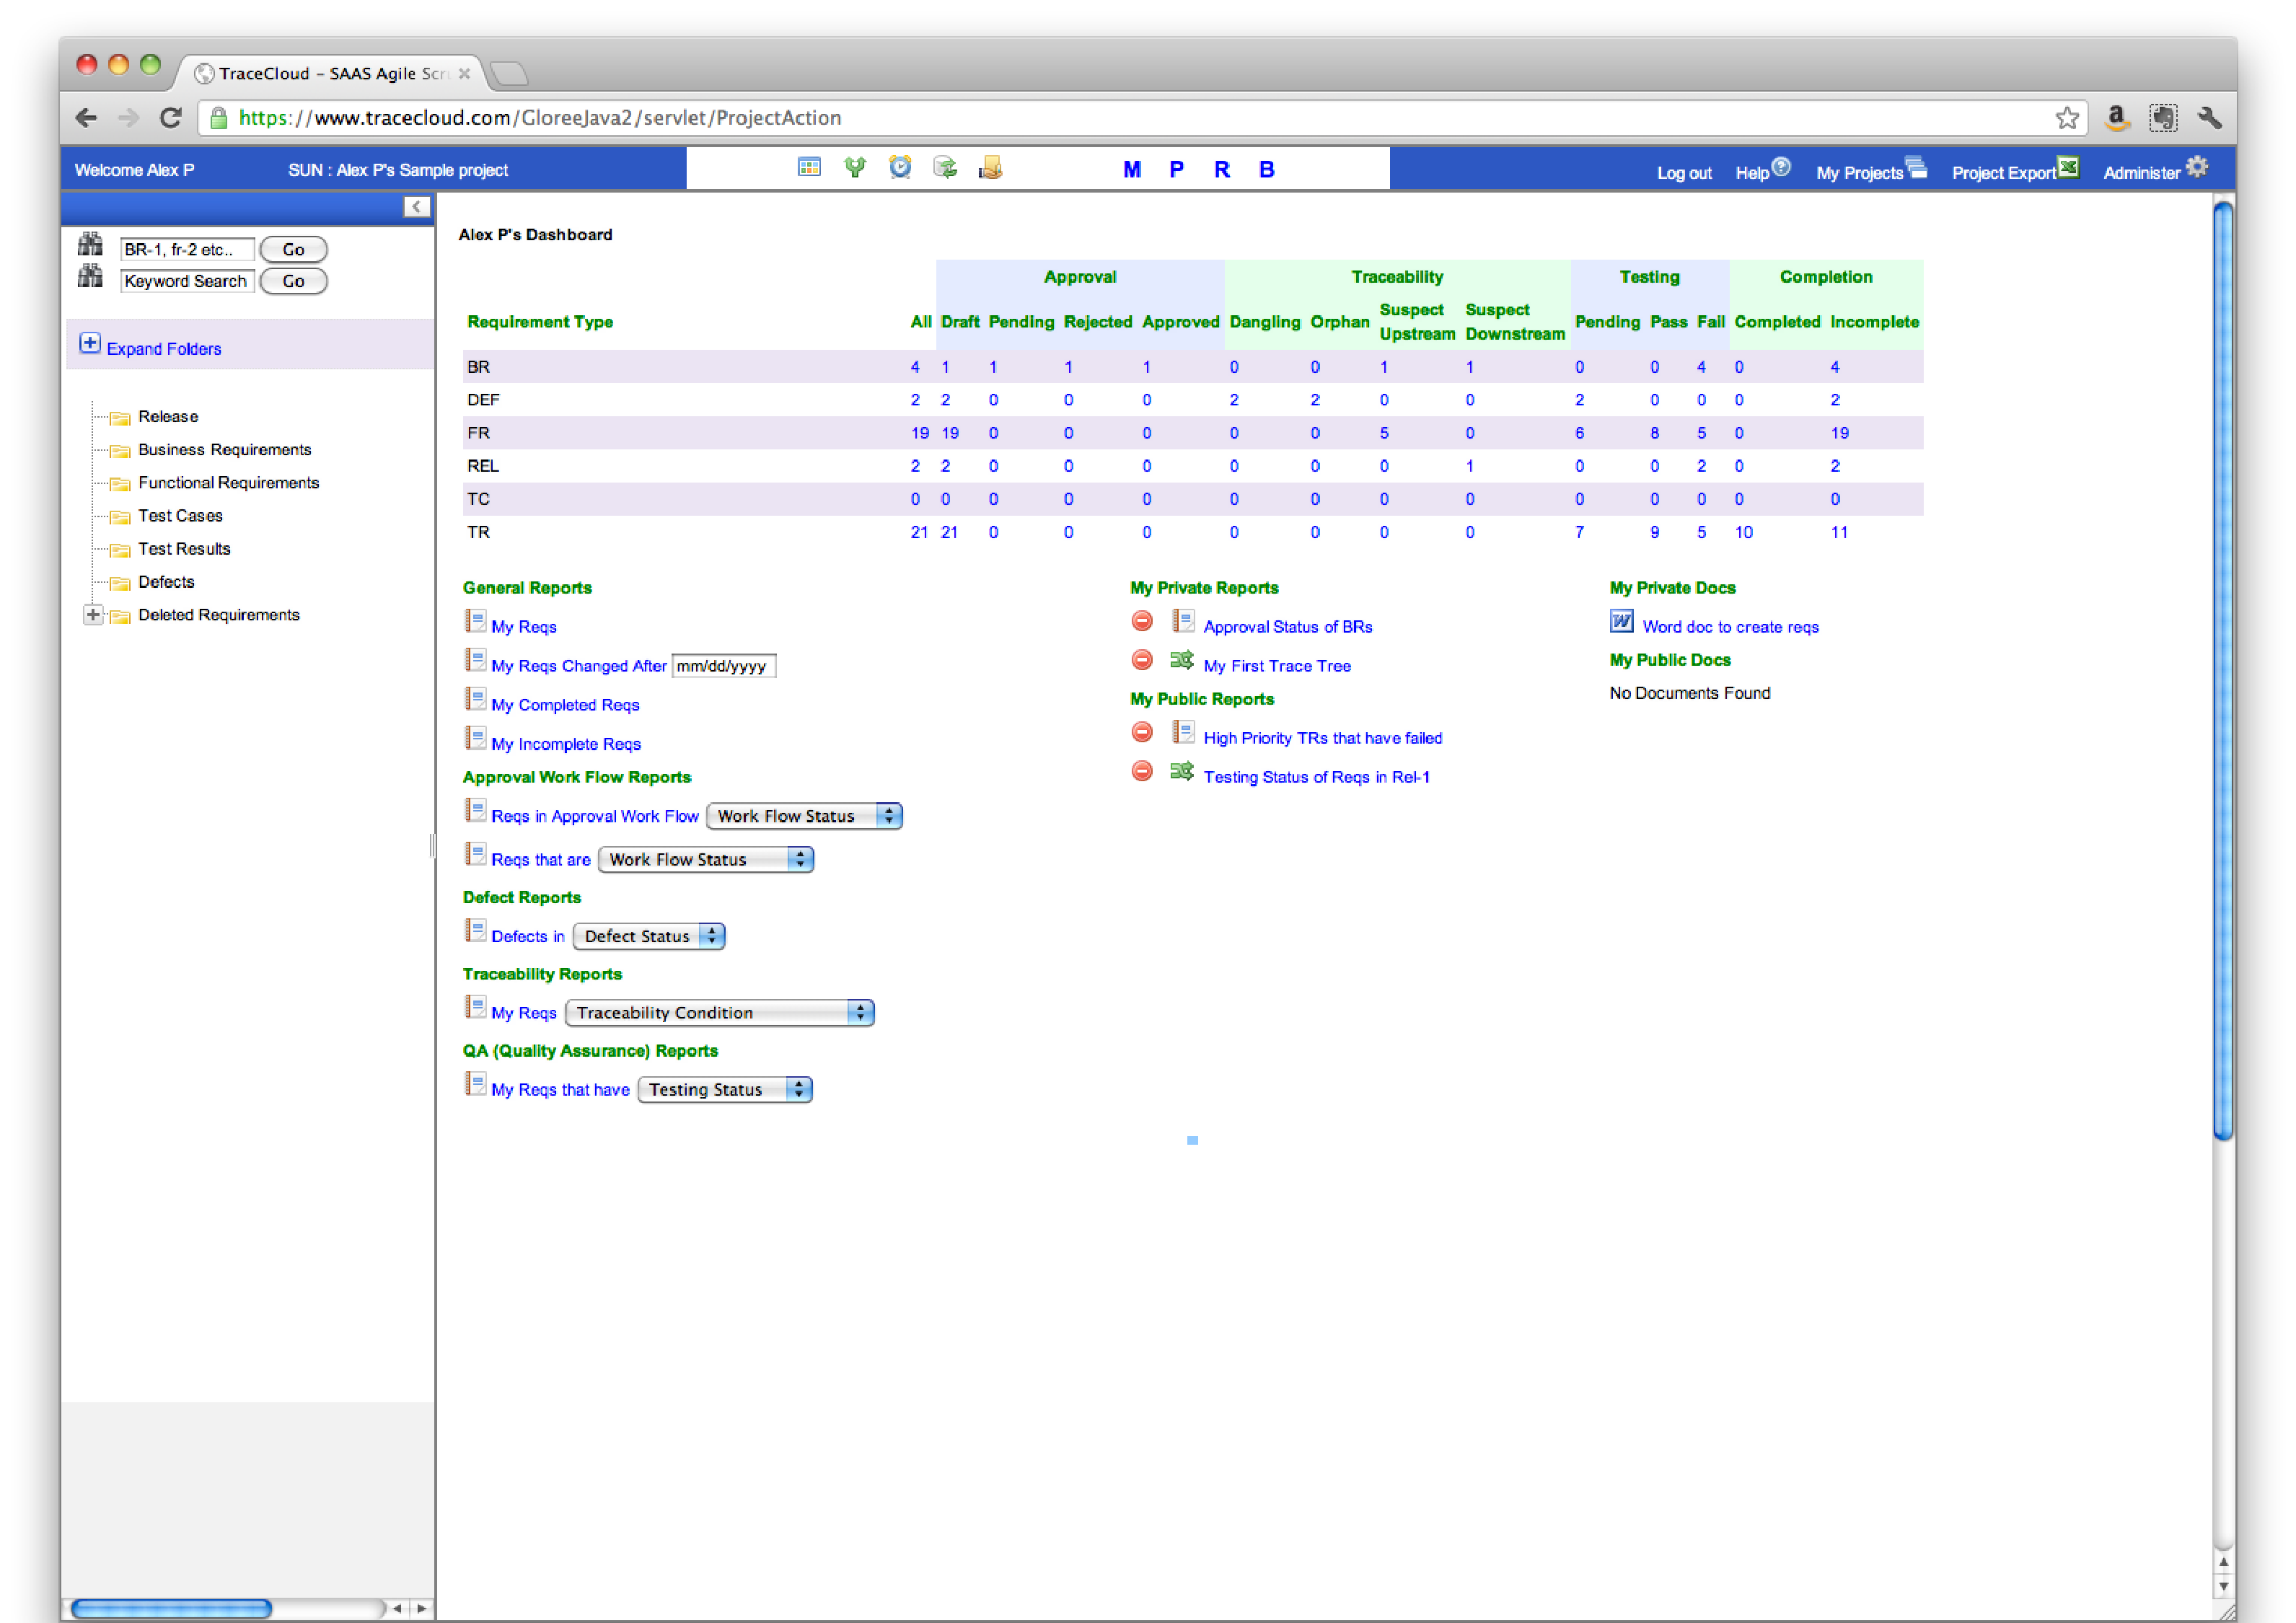
\includegraphics[width=1.0\textwidth]{img/tracecloud_2.pdf}
          \caption{Tracecloud - ekran główny}
          \label{fig:tracecloud_2}
        \end{figure*}

        \begin{figure*}[t]
          \centering
          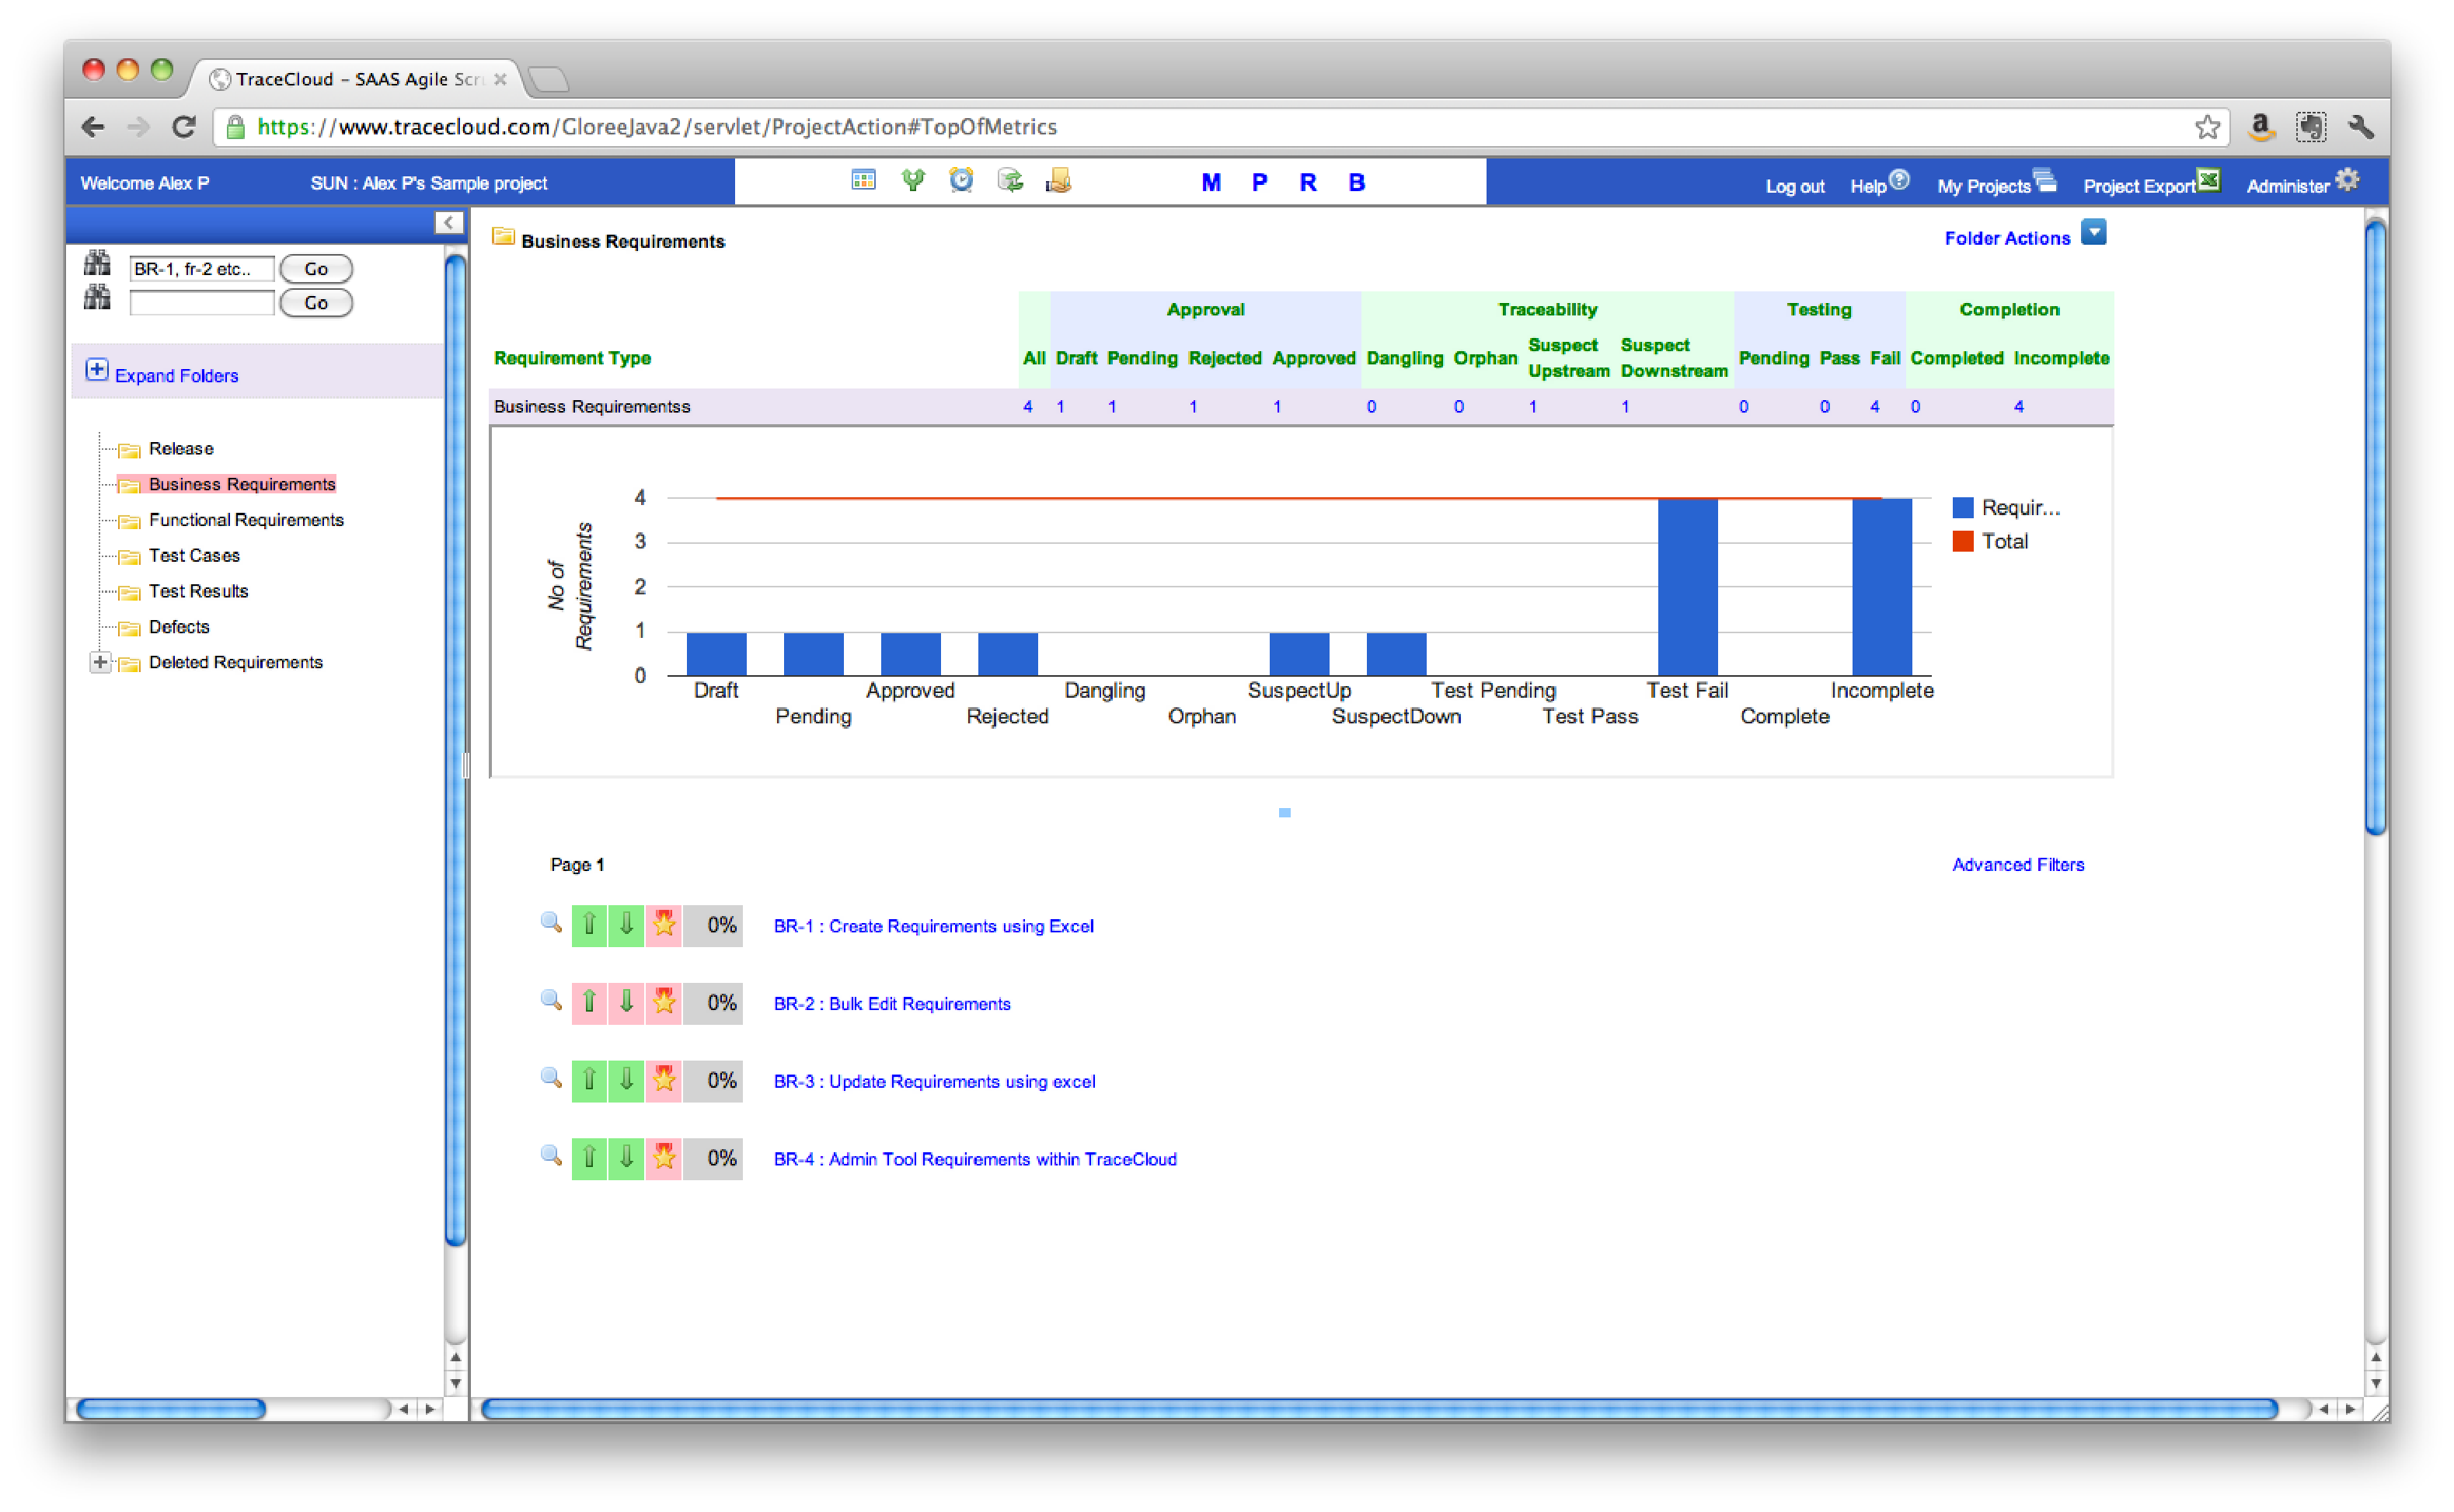
\includegraphics[width=1.0\textwidth]{img/tracecloud_3.pdf}
          \caption{Tracecloud - przegląd wymagań}
          \label{fig:tracecloud_3}
        \end{figure*}

        \begin{figure*}[t]
          \centering
          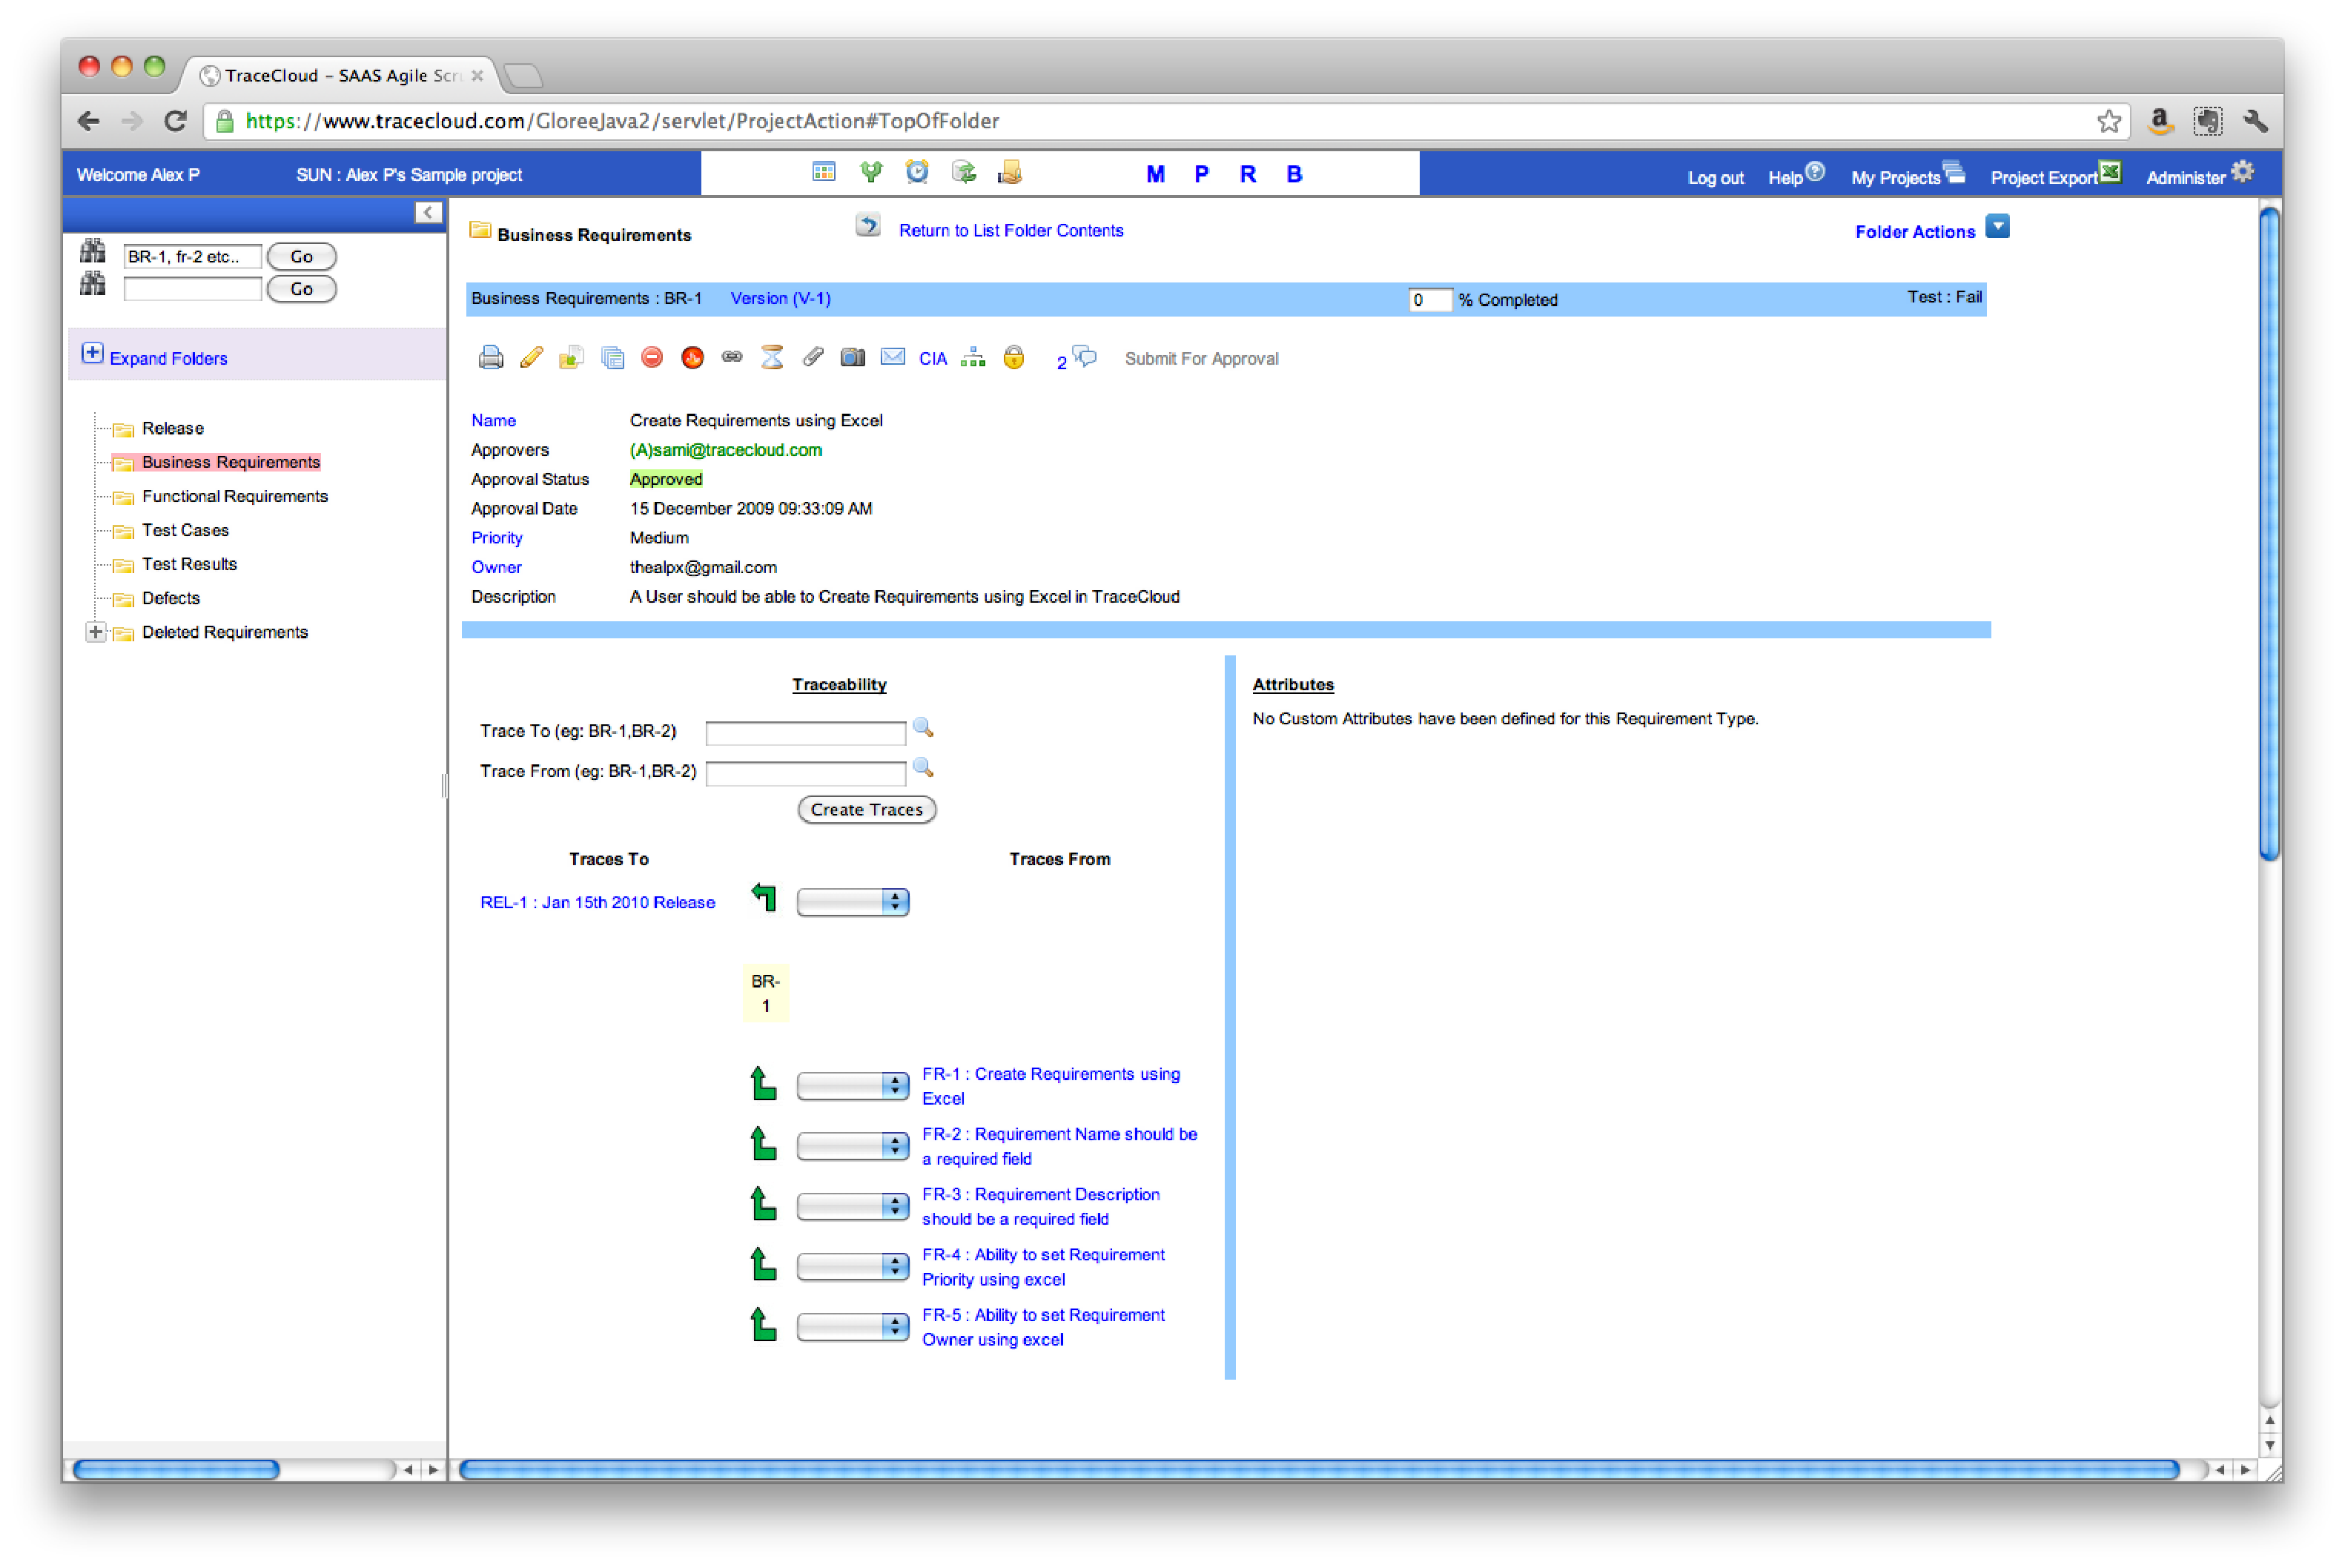
\includegraphics[width=1.0\textwidth]{img/tracecloud_4.pdf}
          \caption{Tracecloud - szczegóły wymagania}
          \label{fig:tracecloud_4}
        \end{figure*}

      \subsubsection{Tracecloud}
        
        Jak widać na rys. \ref{fig:tracecloud_1} Tracecloud jest znacznie gorzej przygotowany od strony interfejsu użytkownika. Mimo tego jest znacznie bardziej skompilkowanym systemem, udostępniającym znacznie więcej funkcjonalności niż Gatherspace.

        Główny przegląd projektu zawiera tabelę z wyświetlonymi metrykami projektu. Można z niej odczytać ilość zaimplementowanych wymagań, ilościowe wyniki testów, przedląd zgłoszonych błędów i wartości liczbowe wymagań pogrupowane w poszczególne statusy. Po dokładnym przeanalizowaniu tabeli, można odczytać interesujące informacje na temat projektu, jednak użyteczność tego sposobu reprezentacji stanu projektu jest bardzo niska. 

        Oprócz ilościowego przeglądu stanu projektu, użytkownik ma do dyspozycji menu i odnośniki do najważniejszych modułów systemu, taki jak wymagania biznesowe, funkcjonalne, scenariusze testowe i błędy.

        Przegląd wymagań opiera się o wykres ze statystykami oraz prostą listę (rys. \ref{fig:tracecloud_3}), z kolei szczegóły wymagania zawierają informację o jego nazwie, priorytecie, właścicielu oraz opis. Dodatkowo twórcy umieścili moduł śledzenia umożliwiający połączenie wymagań biznesowych z funkcjonalnymi (rys. \ref{fig:tracecloud_4}).
    
        Oprócz licznych raportów wyświetlanych w obrębie aplikacji, nie znaleziono funkcjonalności generowania dokmentu specyfikacji wymagań. 

        Tracecloud dostępny jest jako wersja Trial przez 6 miesięcy. Koszt wdrożenia waha się od 350\$ do 1000\$ za miesiąc użytkownania systemu w zależności od maksymalnej ilości obsługiwanych wymagań. Najtańsza licencja przewiduje obsługę do 5000 wymagań, podczas gdy wersja najdroższa - do 10tyś.

    \subsection{Aplikacje desktopowe}

      Model SaaS, mimo wszystkich swoich zalet, posiada również wady. Głównym powodem kontrowersji jest konieczność powierzenia danych biznesowych firmie udostępniającej narzędzie na swoich serwerach. Dla dużych korporacji, pilnie strzegących swoich tajemnic handlowych, takie rozwiązanie, może być nie do zaakceptowania ze względów bezpieczeństwa. Mimo potencjalnej możliwośći uniknięcia kosztów budowy i utrzymania infrastruktury sprzętowo-software'owej ryzyko związane z brakiem kontroli nad powierzonymi danymi jest często zbyt wielkie. 

      W klasycznych aplikacjach okienkowych, odpowiedzialność w zakresie zabezpieczenia danych spoczywa na samej korporacji i jej pracowniku. Dzięki temu, nadal istnieje zapotrzebowanie na oprogramowanie instalowane na lokalnym dysku użytkownika. Przykładami takich aplikacji są m.in. IBM DOORS oraz IBM Rational Requirements Composer.

      \subsubsection{RequisitePRO}
      \subsubsection{DOORS}

    \subsection{Platforma IBM .jazz}

      Platforma IBM jazz zasługuje na osobną sekcję, ponieważ jest zintegrowanym, kompleksowym zestawem narzędzi i aplikacji dla przedsiębiorstw tworzących oprogramowanie. Centrum zarządzania platformą jazz jest serwer stanowiący repozytorium danych i ośrodek dowodzenia. Platforma składa się zarówno udostępnionych na serwerze usług sieciowych oraz aplikacji instalowanych lokalnie, łączących się ze zdalnym serwerem (tzw. rich-client applications). 

  \section{Problemy z istniejącymi rozwiązaniami}

      Analizując istniejące rozwiązania, nie można oprzeć się wrażeniu, że wszystkie przystosowane są do dużych, korporacyjnych projektów. Większość aplikacji powiela rozwiązania znane i sprawdzone funkcjonalności. W konsekwencji trudnym zadaniem jest znalezienie wyróżniających się elementów wśród oferowanych możliwości tych produktów. Wyróżniają się szczególnie ciężkie aplikacje desktopowe od firmy IBM, jednak są one przystosowane do bardzo dużych projektów. Małe i średnie przedsiębiorstwa potrzebują prostszych i ,,lżejszych rozwiązań''. 

      Proces definiowania wymagań w niewielkich projektach jest w dużej mierze procesem twórczym. Często pojawienie się nowego wymagania jest inicjowane z kilku heterogenicznych źródeł. Nierzadko zdarza się również, że to samo wymaganie jest różnie komunikowane przez wiele źródeł. W niewielkich projektach, gdzie często jedna osoba, lub mały zespół odpowiedzialny jest za specyfikację wymagań, wymagania przybierają postać wiadomości email, rozmów telefonicznych, notatek ze spotkań i formalnych dokumentów. Zadaniem osoby lub zespołu odpowiedzialnego za specyfikację wymagań, jest przefiltrowanie cząstkowych informacji oraz ekstrakcja i udokumentowanie wymagań. Żadne narzędzie (przynajmniej na razie) nie zastąpi skutecznie pracy człowieka nad wyłuskaniem wszystkich wymagań. 
